\documentclass[twoside]{book}

% Packages required by doxygen
\usepackage{fixltx2e}
\usepackage{calc}
\usepackage{doxygen}
\usepackage{graphicx}
\usepackage[utf8]{inputenc}
\usepackage{makeidx}
\usepackage{multicol}
\usepackage{multirow}
\PassOptionsToPackage{warn}{textcomp}
\usepackage{textcomp}
\usepackage[nointegrals]{wasysym}
\usepackage[table]{xcolor}

% NLS support packages
\usepackage[catalan]{babel}

% Font selection
\usepackage[T1]{fontenc}
\usepackage{mathptmx}
\usepackage[scaled=.90]{helvet}
\usepackage{courier}
\usepackage{amssymb}
\usepackage{sectsty}
\renewcommand{\familydefault}{\sfdefault}
\allsectionsfont{%
  \fontseries{bc}\selectfont%
  \color{darkgray}%
}
\renewcommand{\DoxyLabelFont}{%
  \fontseries{bc}\selectfont%
  \color{darkgray}%
}
\newcommand{\+}{\discretionary{\mbox{\scriptsize$\hookleftarrow$}}{}{}}

% Page & text layout
\usepackage{geometry}
\geometry{%
  a4paper,%
  top=2.5cm,%
  bottom=2.5cm,%
  left=2.5cm,%
  right=2.5cm%
}
\tolerance=750
\hfuzz=15pt
\hbadness=750
\setlength{\emergencystretch}{15pt}
\setlength{\parindent}{0cm}
\setlength{\parskip}{0.2cm}
\makeatletter
\renewcommand{\paragraph}{%
  \@startsection{paragraph}{4}{0ex}{-1.0ex}{1.0ex}{%
    \normalfont\normalsize\bfseries\SS@parafont%
  }%
}
\renewcommand{\subparagraph}{%
  \@startsection{subparagraph}{5}{0ex}{-1.0ex}{1.0ex}{%
    \normalfont\normalsize\bfseries\SS@subparafont%
  }%
}
\makeatother

% Headers & footers
\usepackage{fancyhdr}
\pagestyle{fancyplain}
\fancyhead[LE]{\fancyplain{}{\bfseries\thepage}}
\fancyhead[CE]{\fancyplain{}{}}
\fancyhead[RE]{\fancyplain{}{\bfseries\leftmark}}
\fancyhead[LO]{\fancyplain{}{\bfseries\rightmark}}
\fancyhead[CO]{\fancyplain{}{}}
\fancyhead[RO]{\fancyplain{}{\bfseries\thepage}}
\fancyfoot[LE]{\fancyplain{}{}}
\fancyfoot[CE]{\fancyplain{}{}}
\fancyfoot[RE]{\fancyplain{}{\bfseries\scriptsize Generat a Dt Mai 31 2016 14\+:37\+:31 per a Pràctica P\+R\+O2 per Doxygen }}
\fancyfoot[LO]{\fancyplain{}{\bfseries\scriptsize Generat a Dt Mai 31 2016 14\+:37\+:31 per a Pràctica P\+R\+O2 per Doxygen }}
\fancyfoot[CO]{\fancyplain{}{}}
\fancyfoot[RO]{\fancyplain{}{}}
\renewcommand{\footrulewidth}{0.4pt}
\renewcommand{\chaptermark}[1]{%
  \markboth{#1}{}%
}
\renewcommand{\sectionmark}[1]{%
  \markright{\thesection\ #1}%
}

% Indices & bibliography
\usepackage{natbib}
\usepackage[titles]{tocloft}
\setcounter{tocdepth}{3}
\setcounter{secnumdepth}{5}
\makeindex

% Hyperlinks (required, but should be loaded last)
\usepackage{ifpdf}
\ifpdf
  \usepackage[pdftex,pagebackref=true]{hyperref}
\else
  \usepackage[ps2pdf,pagebackref=true]{hyperref}
\fi
\hypersetup{%
  colorlinks=true,%
  linkcolor=blue,%
  citecolor=blue,%
  unicode%
}

% Custom commands
\newcommand{\clearemptydoublepage}{%
  \newpage{\pagestyle{empty}\cleardoublepage}%
}


%===== C O N T E N T S =====

\begin{document}

% Titlepage & ToC
\hypersetup{pageanchor=false,
             bookmarks=true,
             bookmarksnumbered=true,
             pdfencoding=unicode
            }
\pagenumbering{roman}
\begin{titlepage}
\vspace*{7cm}
\begin{center}%
{\Large Pràctica P\+R\+O2 \\[1ex]\large version 1 31-\/may-\/2016 }\\
\vspace*{1cm}
{\large Generat per Doxygen 1.8.8}\\
\vspace*{0.5cm}
{\small Dt Mai 31 2016 14:37:31}\\
\end{center}
\end{titlepage}
\clearemptydoublepage
\tableofcontents
\clearemptydoublepage
\pagenumbering{arabic}
\hypersetup{pageanchor=true}

%--- Begin generated contents ---
\chapter{Índex de Classes}
\section{Llista de Classes}
Aquestes són les classes, estructures, unions i interfícies acompanyades amb breus descripcions\+:\begin{DoxyCompactList}
\item\contentsline{section}{\hyperlink{class_cites}{Cites} \\*Gestionador de cites }{\pageref{class_cites}}{}
\item\contentsline{section}{\hyperlink{class_cjt__autors}{Cjt\+\_\+autors} \\*Conjunt d'autors amb textos i cites }{\pageref{class_cjt__autors}}{}
\item\contentsline{section}{\hyperlink{class_text}{Text} \\*\hyperlink{class_text}{Text} }{\pageref{class_text}}{}
\end{DoxyCompactList}

\chapter{Índex de Fitxers}
\section{Llista dels Fitxers}
Aquesta és la llista de tots els fitxers acompanyats amb breus descripcions\+:\begin{DoxyCompactList}
\item\contentsline{section}{\hyperlink{_cites_8cc}{Cites.\+cc} }{\pageref{_cites_8cc}}{}
\item\contentsline{section}{\hyperlink{_cites_8hh}{Cites.\+hh} \\*Especificació de la clase \hyperlink{class_cites}{Cites} }{\pageref{_cites_8hh}}{}
\item\contentsline{section}{\hyperlink{_cjt__autors_8cc}{Cjt\+\_\+autors.\+cc} }{\pageref{_cjt__autors_8cc}}{}
\item\contentsline{section}{\hyperlink{_cjt__autors_8hh}{Cjt\+\_\+autors.\+hh} \\*Especificació de la clase \hyperlink{class_cjt__autors}{Cjt\+\_\+autors} }{\pageref{_cjt__autors_8hh}}{}
\item\contentsline{section}{\hyperlink{program_8cc}{program.\+cc} }{\pageref{program_8cc}}{}
\item\contentsline{section}{\hyperlink{_text_8cc}{Text.\+cc} }{\pageref{_text_8cc}}{}
\item\contentsline{section}{\hyperlink{_text_8hh}{Text.\+hh} \\*Especificació de la clase \hyperlink{class_text}{Text} }{\pageref{_text_8hh}}{}
\end{DoxyCompactList}

\chapter{Documentació de les Classes}
\hypertarget{class_cites}{\section{Referència de la Classe Cites}
\label{class_cites}\index{Cites@{Cites}}
}


Gestionador de cites.  


\subsection*{Mètodes públics}
\begin{DoxyCompactItemize}
\item 
\hyperlink{class_cites_aef7c40360c5537b4dac136a758e815fc}{Cites} ()
\begin{DoxyCompactList}\small\item\em Invariant de la representació\+: \end{DoxyCompactList}\item 
\hyperlink{class_cites_a7cbea31abf7bb3aeaae56592545c2390}{$\sim$\+Cites} ()
\begin{DoxyCompactList}\small\item\em Constructora de la classe. \end{DoxyCompactList}\item 
void \hyperlink{class_cites_a66ce36e7002b77e08ab58c865c6538dd}{afegir\+\_\+cita} (int frase\+\_\+inicial, int frase\+\_\+final, vector$<$ string $>$ frases, string nom\+\_\+autor, string titol\+\_\+text)
\item 
void \hyperlink{class_cites_a001083c304cb7d6305bde75dd4cb28fe}{eliminar\+\_\+cita} (string referencia)
\begin{DoxyCompactList}\small\item\em Mètode per afegir una cita. \end{DoxyCompactList}\item 
void \hyperlink{class_cites_af2f27446487bb2763199cf35e45bc9b3}{imprimir\+\_\+cita} (string referencia)
\begin{DoxyCompactList}\small\item\em Mètode per consultar les inicials d'un autor. \end{DoxyCompactList}\item 
void \hyperlink{class_cites_a780d46001297c44f21f0acc827ffe651}{imprimir\+\_\+cites\+\_\+autor} (string nom\+\_\+autor)
\begin{DoxyCompactList}\small\item\em Mètode per imprimir una cita. \end{DoxyCompactList}\item 
void \hyperlink{class_cites_a3491d06f3db170f20a719fd05c132200}{imprimir\+\_\+cites\+\_\+text} (string titol\+\_\+text)
\begin{DoxyCompactList}\small\item\em Mètode per imprimir les cites d'un autor. \end{DoxyCompactList}\item 
void \hyperlink{class_cites_ac6bfa4ddde0539469b662515b61212bc}{imprimir\+\_\+cites\+\_\+associades} (string titol\+\_\+text)
\begin{DoxyCompactList}\small\item\em Mètode per imprimir les cites d'un text. \end{DoxyCompactList}\item 
void \hyperlink{class_cites_afaa3bf8137743be02fa0dea30b7cd9bb}{imprimir\+\_\+totes\+\_\+cites} ()
\begin{DoxyCompactList}\small\item\em Mètode per imprimir cites associades. \end{DoxyCompactList}\end{DoxyCompactItemize}
\subsection*{Mètodes Públics Estàtics}
\begin{DoxyCompactItemize}
\item 
static string \hyperlink{class_cites_aef796d574e43afc5830b8825e711f50f}{inicials\+\_\+autor} (string autor)
\begin{DoxyCompactList}\small\item\em Mètode per eliminar una cita. \end{DoxyCompactList}\end{DoxyCompactItemize}


\subsection{Descripció Detallada}
Gestionador de cites. 

Definició a la línia 18 del fitxer Cites.\+hh.



\subsection{Documentació del Constructor i el Destructor}
\hypertarget{class_cites_aef7c40360c5537b4dac136a758e815fc}{\index{Cites@{Cites}!Cites@{Cites}}
\index{Cites@{Cites}!Cites@{Cites}}
\subsubsection[{Cites}]{\setlength{\rightskip}{0pt plus 5cm}Cites\+::\+Cites (
\begin{DoxyParamCaption}
{}
\end{DoxyParamCaption}
)}}\label{class_cites_aef7c40360c5537b4dac136a758e815fc}


Invariant de la representació\+: 


\begin{DoxyItemize}
\item cites és un diccionari que conté la referència completa (inicials de l'autor + índex) de cada cita i la pròpia cita. Les referències no es poden repetir i l'índex començarà a 1
\item referencies és un diccionari que utilitza les inicials del autor de la cita referenciada amb un comptador com a objecte que compta el nombre de vegades que han aparegut aquestes inicials des de l'inici del programa 
\end{DoxyItemize}

Definició a la línia 3 del fitxer Cites.\+cc.


\begin{DoxyCode}
3 \{\}
\end{DoxyCode}
\hypertarget{class_cites_a7cbea31abf7bb3aeaae56592545c2390}{\index{Cites@{Cites}!````~Cites@{$\sim$\+Cites}}
\index{````~Cites@{$\sim$\+Cites}!Cites@{Cites}}
\subsubsection[{$\sim$\+Cites}]{\setlength{\rightskip}{0pt plus 5cm}Cites\+::$\sim$\+Cites (
\begin{DoxyParamCaption}
{}
\end{DoxyParamCaption}
)}}\label{class_cites_a7cbea31abf7bb3aeaae56592545c2390}


Constructora de la classe. 

\begin{DoxyPrecond}{Precondició}
Cert 
\end{DoxyPrecond}
\begin{DoxyPostcond}{Postcondició}
El resultat és un gestionador de cites 
\end{DoxyPostcond}


Definició a la línia 120 del fitxer Cites.\+cc.


\begin{DoxyCode}
120 \{\}\end{DoxyCode}


\subsection{Documentació de les Funcions Membre}
\hypertarget{class_cites_a66ce36e7002b77e08ab58c865c6538dd}{\index{Cites@{Cites}!afegir\+\_\+cita@{afegir\+\_\+cita}}
\index{afegir\+\_\+cita@{afegir\+\_\+cita}!Cites@{Cites}}
\subsubsection[{afegir\+\_\+cita}]{\setlength{\rightskip}{0pt plus 5cm}void Cites\+::afegir\+\_\+cita (
\begin{DoxyParamCaption}
\item[{int}]{frase\+\_\+inicial, }
\item[{int}]{frase\+\_\+final, }
\item[{vector$<$ string $>$}]{frases, }
\item[{string}]{nom\+\_\+autor, }
\item[{string}]{titol\+\_\+text}
\end{DoxyParamCaption}
)}}\label{class_cites_a66ce36e7002b77e08ab58c865c6538dd}


Definició a la línia 5 del fitxer Cites.\+cc.


\begin{DoxyCode}
5                                                                                                            
                 \{
6     cita c;
7     c.autor = nom\_autor;
8     c.titol\_text = titol\_text;
9     c.frase\_inicial = frase\_inicial;
10     c.frase\_final = frase\_final;
11     c.frases = frases;
12     \textcolor{keywordtype}{string} referencia = \hyperlink{class_cites_aef796d574e43afc5830b8825e711f50f}{Cites::inicials\_autor}(nom\_autor);
13     map<string, int>::iterator i = referencies.find(referencia);
14     \textcolor{keywordflow}{if} (i == referencies.end()) \{
15         referencies.insert(make\_pair(referencia,1));
16         cites.insert(make\_pair(referencia+\textcolor{charliteral}{'1'},c));
17     \}
18     \textcolor{keywordflow}{else} \{
19         \textcolor{keywordtype}{bool} error = \textcolor{keyword}{false};
20         \textcolor{keywordflow}{for} (\textcolor{keywordtype}{int} n = 0; n < (*i).second+1; n++) \{
21             stringstream nref;
22             nref << n;
23             \textcolor{keywordtype}{string} aux = referencia + nref.str();
24             map<string, cita>::iterator it = cites.find(aux);
25             \textcolor{keywordflow}{if} (it != cites.end() && ((*it).second.titol\_text == titol\_text and (*it).second.frase\_inicial 
      == frase\_inicial and (*it).second.frase\_final == frase\_final))\{
26                 cout << \textcolor{stringliteral}{"error"} << endl;
27                 n = (*i).second+1;
28                 error = \textcolor{keyword}{true};
29             \}
30         \}
31         \textcolor{keywordflow}{if} (not error)\{
32             (*i).second++;
33             stringstream nref;
34             nref << (*i).second;
35             referencia += nref.str();
36             cites.insert(make\_pair(referencia,c));
37         \}
38     \}
39 \}
\end{DoxyCode}
\hypertarget{class_cites_a001083c304cb7d6305bde75dd4cb28fe}{\index{Cites@{Cites}!eliminar\+\_\+cita@{eliminar\+\_\+cita}}
\index{eliminar\+\_\+cita@{eliminar\+\_\+cita}!Cites@{Cites}}
\subsubsection[{eliminar\+\_\+cita}]{\setlength{\rightskip}{0pt plus 5cm}void Cites\+::eliminar\+\_\+cita (
\begin{DoxyParamCaption}
\item[{string}]{referencia}
\end{DoxyParamCaption}
)}}\label{class_cites_a001083c304cb7d6305bde75dd4cb28fe}


Mètode per afegir una cita. 

\begin{DoxyPrecond}{Precondició}
Cert 
\end{DoxyPrecond}
\begin{DoxyPostcond}{Postcondició}
S'ha afegit una cita amb les dades passades pels paràmetres al paràmetre implícit 
\end{DoxyPostcond}


Definició a la línia 41 del fitxer Cites.\+cc.


\begin{DoxyCode}
41                                            \{
42     map<string, cita>::iterator it = cites.find(referencia);
43     \textcolor{keywordflow}{if} (it == cites.end())
44         cout << \textcolor{stringliteral}{"error"} << endl;
45     \textcolor{keywordflow}{else}
46         cites.erase(it);
47 \}
\end{DoxyCode}
\hypertarget{class_cites_aef796d574e43afc5830b8825e711f50f}{\index{Cites@{Cites}!inicials\+\_\+autor@{inicials\+\_\+autor}}
\index{inicials\+\_\+autor@{inicials\+\_\+autor}!Cites@{Cites}}
\subsubsection[{inicials\+\_\+autor}]{\setlength{\rightskip}{0pt plus 5cm}string Cites\+::inicials\+\_\+autor (
\begin{DoxyParamCaption}
\item[{string}]{autor}
\end{DoxyParamCaption}
)\hspace{0.3cm}{\ttfamily [static]}}}\label{class_cites_aef796d574e43afc5830b8825e711f50f}


Mètode per eliminar una cita. 

\begin{DoxyPrecond}{Precondició}
Referencia és la referència vàlida d'una cita existent 
\end{DoxyPrecond}
\begin{DoxyPostcond}{Postcondició}
S'ha eliminat la cita amb referència referencia 
\end{DoxyPostcond}


Definició a la línia 110 del fitxer Cites.\+cc.


\begin{DoxyCode}
110                                         \{
111     stringstream ss;
112     ss << autor;
113     \textcolor{keywordtype}{string} word;
114     \textcolor{keywordtype}{string} inicials;
115     \textcolor{keywordflow}{while} (ss >> word)
116         inicials += word[0];
117     \textcolor{keywordflow}{return} inicials;
118 \}
\end{DoxyCode}
\hypertarget{class_cites_af2f27446487bb2763199cf35e45bc9b3}{\index{Cites@{Cites}!imprimir\+\_\+cita@{imprimir\+\_\+cita}}
\index{imprimir\+\_\+cita@{imprimir\+\_\+cita}!Cites@{Cites}}
\subsubsection[{imprimir\+\_\+cita}]{\setlength{\rightskip}{0pt plus 5cm}void Cites\+::imprimir\+\_\+cita (
\begin{DoxyParamCaption}
\item[{string}]{referencia}
\end{DoxyParamCaption}
)}}\label{class_cites_af2f27446487bb2763199cf35e45bc9b3}


Mètode per consultar les inicials d'un autor. 

\begin{DoxyPrecond}{Precondició}
autor = nom de l'autor 
\end{DoxyPrecond}
\begin{DoxyPostcond}{Postcondició}
Es retornen les inicials de l'autor 
\end{DoxyPostcond}


Definició a la línia 49 del fitxer Cites.\+cc.


\begin{DoxyCode}
49                                            \{
50   map<string, cita>::const\_iterator i = cites.find(referencia);
51   \textcolor{keywordflow}{if} (i == cites.end())
52         cout << \textcolor{stringliteral}{"error"} << endl;
53     \textcolor{keywordflow}{else} \{
54         cout << (*i).second.autor << \textcolor{stringliteral}{" \(\backslash\)""} << (*i).second.titol\_text << \textcolor{stringliteral}{"\(\backslash\)""} << endl;
55         cout << (*i).second.frase\_inicial << \textcolor{stringliteral}{"-"} << (*i).second.frase\_final << endl;
56         \textcolor{keywordtype}{int} n = (*i).second.frases.size();
57         \textcolor{keywordflow}{for} (\textcolor{keywordtype}{int} k = 0; k < n; k++)
58             cout << (*i).second.frase\_inicial + k << \textcolor{stringliteral}{" "} << (*i).second.frases[k] << endl;
59     \}
60 \}
\end{DoxyCode}
\hypertarget{class_cites_a780d46001297c44f21f0acc827ffe651}{\index{Cites@{Cites}!imprimir\+\_\+cites\+\_\+autor@{imprimir\+\_\+cites\+\_\+autor}}
\index{imprimir\+\_\+cites\+\_\+autor@{imprimir\+\_\+cites\+\_\+autor}!Cites@{Cites}}
\subsubsection[{imprimir\+\_\+cites\+\_\+autor}]{\setlength{\rightskip}{0pt plus 5cm}void Cites\+::imprimir\+\_\+cites\+\_\+autor (
\begin{DoxyParamCaption}
\item[{string}]{nom\+\_\+autor}
\end{DoxyParamCaption}
)}}\label{class_cites_a780d46001297c44f21f0acc827ffe651}


Mètode per imprimir una cita. 

\begin{DoxyPrecond}{Precondició}
referencia és la referència vàlida d'una cita existent 
\end{DoxyPrecond}
\begin{DoxyPostcond}{Postcondició}
S'ha imprès la cita amb referència referencia al canal estàndard de sortida 
\end{DoxyPostcond}


Definició a la línia 73 del fitxer Cites.\+cc.


\begin{DoxyCode}
73                                                  \{
74   \textcolor{keywordflow}{for} (map<string, cita>::const\_iterator i = cites.begin(); i != cites.end(); i++) \{
75     \textcolor{keywordflow}{if} ((*i).second.autor == nom\_autor) \{
76       cout << (*i).first << endl;
77       \textcolor{keywordtype}{int} n = (*i).second.frases.size();
78             \textcolor{keywordflow}{for} (\textcolor{keywordtype}{int} k = 0; k < n; k++)
79                 cout << (*i).second.frase\_inicial + k << \textcolor{stringliteral}{" "} << (*i).second.frases[k] << endl;
80       cout << \textcolor{stringliteral}{"\(\backslash\)""} << (*i).second.titol\_text << \textcolor{stringliteral}{"\(\backslash\)""} << endl;
81     \}
82   \}
83 \}
\end{DoxyCode}
\hypertarget{class_cites_a3491d06f3db170f20a719fd05c132200}{\index{Cites@{Cites}!imprimir\+\_\+cites\+\_\+text@{imprimir\+\_\+cites\+\_\+text}}
\index{imprimir\+\_\+cites\+\_\+text@{imprimir\+\_\+cites\+\_\+text}!Cites@{Cites}}
\subsubsection[{imprimir\+\_\+cites\+\_\+text}]{\setlength{\rightskip}{0pt plus 5cm}void Cites\+::imprimir\+\_\+cites\+\_\+text (
\begin{DoxyParamCaption}
\item[{string}]{titol\+\_\+text}
\end{DoxyParamCaption}
)}}\label{class_cites_a3491d06f3db170f20a719fd05c132200}


Mètode per imprimir les cites d'un autor. 

\begin{DoxyPrecond}{Precondició}
Cert 
\end{DoxyPrecond}
\begin{DoxyPostcond}{Postcondició}
s'han imprès totes les cites de l'autor amb nom nom\+\_\+autor, si existeix 
\end{DoxyPostcond}


Definició a la línia 85 del fitxer Cites.\+cc.


\begin{DoxyCode}
85                                                  \{
86     map<string, cita>::iterator i = cites.begin();
87     \textcolor{keywordflow}{while} (i != cites.end()) \{
88     \textcolor{keywordflow}{if} ((*i).second.titol\_text == titol\_text) \{
89             cout << (*i).first << endl;
90       \textcolor{keywordtype}{int} n = (*i).second.frases.size();
91       \textcolor{keywordflow}{for} (\textcolor{keywordtype}{int} k = 0; k < n; k++)
92           cout << (*i).second.frase\_inicial +k << \textcolor{stringliteral}{" "} << (*i).second.frases[k] << endl;
93             cout << (*i).second.autor << \textcolor{stringliteral}{" \(\backslash\)""} << (*i).second.titol\_text << \textcolor{stringliteral}{"\(\backslash\)""} << endl;
94     \}
95     i++;
96   \}
97 \}
\end{DoxyCode}
\hypertarget{class_cites_ac6bfa4ddde0539469b662515b61212bc}{\index{Cites@{Cites}!imprimir\+\_\+cites\+\_\+associades@{imprimir\+\_\+cites\+\_\+associades}}
\index{imprimir\+\_\+cites\+\_\+associades@{imprimir\+\_\+cites\+\_\+associades}!Cites@{Cites}}
\subsubsection[{imprimir\+\_\+cites\+\_\+associades}]{\setlength{\rightskip}{0pt plus 5cm}void Cites\+::imprimir\+\_\+cites\+\_\+associades (
\begin{DoxyParamCaption}
\item[{string}]{titol\+\_\+text}
\end{DoxyParamCaption}
)}}\label{class_cites_ac6bfa4ddde0539469b662515b61212bc}


Mètode per imprimir les cites d'un text. 

\begin{DoxyPrecond}{Precondició}
titol\+\_\+text és el títol d'un text 
\end{DoxyPrecond}
\begin{DoxyPostcond}{Postcondició}
S'han imprès totes les cites del text amb títol titol\+\_\+text 
\end{DoxyPostcond}


Definició a la línia 62 del fitxer Cites.\+cc.


\begin{DoxyCode}
62                                                        \{
63   \textcolor{keywordflow}{for} (map<string, cita>::const\_iterator i = cites.begin(); i != cites.end(); i++) \{
64     \textcolor{keywordflow}{if} ((*i).second.titol\_text == titol\_text) \{
65             cout << (*i).first << endl;
66       \textcolor{keywordtype}{int} n = (*i).second.frases.size();
67       \textcolor{keywordflow}{for} (\textcolor{keywordtype}{int} k = 0; k < n; k++)
68           cout << (*i).second.frase\_inicial +k << \textcolor{stringliteral}{" "} << (*i).second.frases[k] << endl;;
69     \}
70   \}
71 \}
\end{DoxyCode}
\hypertarget{class_cites_afaa3bf8137743be02fa0dea30b7cd9bb}{\index{Cites@{Cites}!imprimir\+\_\+totes\+\_\+cites@{imprimir\+\_\+totes\+\_\+cites}}
\index{imprimir\+\_\+totes\+\_\+cites@{imprimir\+\_\+totes\+\_\+cites}!Cites@{Cites}}
\subsubsection[{imprimir\+\_\+totes\+\_\+cites}]{\setlength{\rightskip}{0pt plus 5cm}void Cites\+::imprimir\+\_\+totes\+\_\+cites (
\begin{DoxyParamCaption}
{}
\end{DoxyParamCaption}
)}}\label{class_cites_afaa3bf8137743be02fa0dea30b7cd9bb}


Mètode per imprimir cites associades. 

\begin{DoxyPrecond}{Precondició}
Cert 
\end{DoxyPrecond}
\begin{DoxyPostcond}{Postcondició}
S'han imprès totes les cites del text amb títol titol\+\_\+text sense el nom de l'autor o el titol del text al final 
\end{DoxyPostcond}


Definició a la línia 99 del fitxer Cites.\+cc.


\begin{DoxyCode}
99                                  \{
100     map<string, cita>::iterator it = cites.begin();
101     \textcolor{keywordflow}{while} (it != cites.end()) \{
102     cout << (*it).first << endl;
103     \textcolor{keywordflow}{for} (\textcolor{keywordtype}{int} i = 0; i < (*it).second.frases.size(); i++)
104             cout << (*it).second.frase\_inicial + i << \textcolor{stringliteral}{" "} << (*it).second.frases[i] << endl;
105         cout << (*it).second.autor << \textcolor{stringliteral}{" \(\backslash\)""} << (*it).second.titol\_text << \textcolor{stringliteral}{"\(\backslash\)""} << endl;
106         it++;
107    \}
108 \}
\end{DoxyCode}


La documentació d'aquesta classe es va generar a partir dels següents fitxers\+:\begin{DoxyCompactItemize}
\item 
\hyperlink{_cites_8hh}{Cites.\+hh}\item 
\hyperlink{_cites_8cc}{Cites.\+cc}\end{DoxyCompactItemize}

\hypertarget{class_cjt__autors}{\section{Referència de la Classe Cjt\+\_\+autors}
\label{class_cjt__autors}\index{Cjt\+\_\+autors@{Cjt\+\_\+autors}}
}


Conjunt d'autors amb textos i cites.  


\subsection*{Mètodes públics}
\begin{DoxyCompactItemize}
\item 
void \hyperlink{class_cjt__autors_a0fb9864fd22881216650552d0697e52d}{comanda} (string comanda)
\item 
\hyperlink{class_cjt__autors_a7ecfc670f529e537c255693f847a8466}{Cjt\+\_\+autors} ()
\begin{DoxyCompactList}\small\item\em Mètode per gestionar les comandes del programa. \end{DoxyCompactList}\item 
\hyperlink{class_cjt__autors_a157ba520241307b0e7156d620b167a04}{$\sim$\+Cjt\+\_\+autors} ()
\begin{DoxyCompactList}\small\item\em Constructora de la classe. \end{DoxyCompactList}\item 
void \hyperlink{class_cjt__autors_a171709e9426f62ecdcd1eba359965028}{eliminar\+\_\+text} ()
\item 
void \hyperlink{class_cjt__autors_a5811a00943aea93a50098d7c2053b9a8}{eliminar\+\_\+cita} ()
\begin{DoxyCompactList}\small\item\em Mètode per eliminar un text. \end{DoxyCompactList}\item 
void \hyperlink{class_cjt__autors_a7033452c9f98edee600a39022dd23c4a}{substituir} ()
\begin{DoxyCompactList}\small\item\em Mètode per eliminar una cita. \end{DoxyCompactList}\item 
void \hyperlink{class_cjt__autors_a5b975fe803a82fe99de5e92e32bcd681}{seleccionar\+\_\+text} ()
\begin{DoxyCompactList}\small\item\em Mètode per substituir paraules en un text. \end{DoxyCompactList}\item 
bool \hyperlink{class_cjt__autors_a60adf6ed96d0c69487bd7e9de6aa7e1d}{hi\+\_\+ha\+\_\+seleccio} ()
\begin{DoxyCompactList}\small\item\em Mètode per seleccionar un text. \end{DoxyCompactList}\item 
void \hyperlink{class_cjt__autors_a9449545eb6877cb96e54d121faff04d1}{frases} ()
\begin{DoxyCompactList}\small\item\em Mètode per saber si hi ha un text seleccionat. \end{DoxyCompactList}\item 
void \hyperlink{class_cjt__autors_a2c0fec1160c25fd7d458ff0b62f250ff}{afegir\+\_\+cita} ()
\begin{DoxyCompactList}\small\item\em Mètode per tractar les comandes que comencen amb \char`\"{}frases\char`\"{}. \end{DoxyCompactList}\item 
void \hyperlink{class_cjt__autors_aec38f4dac32347c8b320bbf4aa204b5b}{afegir\+\_\+text} ()
\begin{DoxyCompactList}\small\item\em Mètode per afegir una cita. \end{DoxyCompactList}\item 
void \hyperlink{class_cjt__autors_a408618804b43301a240b75a9592c77d0}{imprimeix\+\_\+tots\+\_\+textos} ()
\begin{DoxyCompactList}\small\item\em Mètode per afegir un text. \end{DoxyCompactList}\item 
void \hyperlink{class_cjt__autors_a29ee6a7cf456ab121e154b68b0e5ec4c}{imprimeix\+\_\+tots\+\_\+autors} ()
\begin{DoxyCompactList}\small\item\em Mètode per imprimir tots els textos. \end{DoxyCompactList}\item 
void \hyperlink{class_cjt__autors_ae89d39d6a6ba754a3f2442de2b7a56db}{imprimeix\+\_\+tots\+\_\+textos\+\_\+autor} ()
\begin{DoxyCompactList}\small\item\em Mètode per imprimir tots els autors. \end{DoxyCompactList}\item 
void \hyperlink{class_cjt__autors_ac98f1a4d2ec3a115ac089ca33c7a6f9c}{imprimeix\+\_\+info} ()
\begin{DoxyCompactList}\small\item\em Mètode per imprimir tots els textos d'un autor. \end{DoxyCompactList}\item 
void \hyperlink{class_cjt__autors_a84d76f9c9487d5f36c10a6a5b3739de3}{imprimeix\+\_\+info\+\_\+cita} ()
\begin{DoxyCompactList}\small\item\em Mètode per imprimir informació d'un text. \end{DoxyCompactList}\item 
void \hyperlink{class_cjt__autors_a583a23dac0ab39f588aae1df306b7dc3}{imprimeix\+\_\+autor\+\_\+text} ()
\begin{DoxyCompactList}\small\item\em Mètode per imprimir informació d'una cita. \end{DoxyCompactList}\item 
void \hyperlink{class_cjt__autors_a56fbd0fb78bf29adc6525c9d2a6ae117}{imprimeix\+\_\+contingut\+\_\+text} ()
\begin{DoxyCompactList}\small\item\em Mètode per imprimir l'autor d'un text. \end{DoxyCompactList}\item 
void \hyperlink{class_cjt__autors_ad6a8a06f8a706808a133d0c11c579656}{imprimeix\+\_\+nombre\+\_\+frases} ()
\begin{DoxyCompactList}\small\item\em Mètode per imprimir el contingut d'un text. \end{DoxyCompactList}\item 
void \hyperlink{class_cjt__autors_a63c6fd83a2ce3a2bd150237fe9619f8c}{imprimeix\+\_\+nombre\+\_\+paraules} ()
\begin{DoxyCompactList}\small\item\em Mètode per imprimir el nombre de frases. \end{DoxyCompactList}\item 
void \hyperlink{class_cjt__autors_a90b657e80e6cb212a7cbf0f8c05e69d0}{imprimeix\+\_\+taula\+\_\+frequencies} ()
\begin{DoxyCompactList}\small\item\em Mètode per imprimir el nombre de paraules. \end{DoxyCompactList}\item 
void \hyperlink{class_cjt__autors_a388318c22b9aef045e8f6646cfc3b638}{imprimeix\+\_\+totes\+\_\+cites} ()
\begin{DoxyCompactList}\small\item\em Mètode per imprimir la taula de freqûències. \end{DoxyCompactList}\item 
void \hyperlink{class_cjt__autors_ae515dc988d61c3cc44235d72dc6e8482}{imprimeix\+\_\+cites\+\_\+autor} ()
\begin{DoxyCompactList}\small\item\em Mètode per imprimir totes les cites. \end{DoxyCompactList}\item 
void \hyperlink{class_cjt__autors_ab9e4765e7eb501e346eee78fc57d05ea}{imprimeix\+\_\+cites\+\_\+text} ()
\begin{DoxyCompactList}\small\item\em Mètode per imprimir totes les cites d'un autor. \end{DoxyCompactList}\end{DoxyCompactItemize}
\subsection*{Atributs Públics}
\begin{DoxyCompactItemize}
\item 
stringstream \hyperlink{class_cjt__autors_a833753dc5eaa466591f7dce971e5021c}{primera\+\_\+linea}
\begin{DoxyCompactList}\small\item\em Invariant de la representacio\+: \end{DoxyCompactList}\end{DoxyCompactItemize}


\subsection{Descripció Detallada}
Conjunt d'autors amb textos i cites. 

Definició a la línia 14 del fitxer Cjt\+\_\+autors.\+hh.



\subsection{Documentació del Constructor i el Destructor}
\hypertarget{class_cjt__autors_a7ecfc670f529e537c255693f847a8466}{\index{Cjt\+\_\+autors@{Cjt\+\_\+autors}!Cjt\+\_\+autors@{Cjt\+\_\+autors}}
\index{Cjt\+\_\+autors@{Cjt\+\_\+autors}!Cjt\+\_\+autors@{Cjt\+\_\+autors}}
\subsubsection[{Cjt\+\_\+autors}]{\setlength{\rightskip}{0pt plus 5cm}Cjt\+\_\+autors\+::\+Cjt\+\_\+autors (
\begin{DoxyParamCaption}
{}
\end{DoxyParamCaption}
)}}\label{class_cjt__autors_a7ecfc670f529e537c255693f847a8466}


Mètode per gestionar les comandes del programa. 

\begin{DoxyPrecond}{Precondició}
comanda = Comanda 
\end{DoxyPrecond}
\begin{DoxyPostcond}{Postcondició}
Tracta la comanda Comanda 
\end{DoxyPostcond}


Definició a la línia 3 del fitxer Cjt\+\_\+autors.\+cc.


\begin{DoxyCode}
3                        \{
4     seleccio = \textcolor{keyword}{false};
5 \}
\end{DoxyCode}
\hypertarget{class_cjt__autors_a157ba520241307b0e7156d620b167a04}{\index{Cjt\+\_\+autors@{Cjt\+\_\+autors}!````~Cjt\+\_\+autors@{$\sim$\+Cjt\+\_\+autors}}
\index{````~Cjt\+\_\+autors@{$\sim$\+Cjt\+\_\+autors}!Cjt\+\_\+autors@{Cjt\+\_\+autors}}
\subsubsection[{$\sim$\+Cjt\+\_\+autors}]{\setlength{\rightskip}{0pt plus 5cm}Cjt\+\_\+autors\+::$\sim$\+Cjt\+\_\+autors (
\begin{DoxyParamCaption}
{}
\end{DoxyParamCaption}
)}}\label{class_cjt__autors_a157ba520241307b0e7156d620b167a04}


Constructora de la classe. 

\begin{DoxyPrecond}{Precondició}
Cert 
\end{DoxyPrecond}
\begin{DoxyPostcond}{Postcondició}
El resultat es un conjunt d'autors amb els seus textos, buit 
\end{DoxyPostcond}


Definició a la línia 389 del fitxer Cjt\+\_\+autors.\+cc.


\begin{DoxyCode}
389 \{\}\end{DoxyCode}


\subsection{Documentació de les Funcions Membre}
\hypertarget{class_cjt__autors_a0fb9864fd22881216650552d0697e52d}{\index{Cjt\+\_\+autors@{Cjt\+\_\+autors}!comanda@{comanda}}
\index{comanda@{comanda}!Cjt\+\_\+autors@{Cjt\+\_\+autors}}
\subsubsection[{comanda}]{\setlength{\rightskip}{0pt plus 5cm}void Cjt\+\_\+autors\+::comanda (
\begin{DoxyParamCaption}
\item[{string}]{comanda}
\end{DoxyParamCaption}
)}}\label{class_cjt__autors_a0fb9864fd22881216650552d0697e52d}


Definició a la línia 54 del fitxer Cjt\+\_\+autors.\+cc.


\begin{DoxyCode}
54                                        \{
55     \textcolor{keywordtype}{char} useless;
56     cout << comande << endl;
57     \hyperlink{class_cjt__autors_a833753dc5eaa466591f7dce971e5021c}{primera\_linea}.str(\textcolor{stringliteral}{""});
58     \hyperlink{class_cjt__autors_a833753dc5eaa466591f7dce971e5021c}{primera\_linea}.clear();
59     \hyperlink{class_cjt__autors_a833753dc5eaa466591f7dce971e5021c}{primera\_linea} << comande;
60     \textcolor{keywordtype}{string} paraula;
61     \hyperlink{class_cjt__autors_a833753dc5eaa466591f7dce971e5021c}{primera\_linea} >> paraula;
62     \textcolor{keywordflow}{if} (paraula == \textcolor{stringliteral}{"afegir"}) \{
63         \hyperlink{class_cjt__autors_a833753dc5eaa466591f7dce971e5021c}{primera\_linea} >> paraula;
64         \textcolor{keywordflow}{if} (paraula == \textcolor{stringliteral}{"text"})
65             \hyperlink{class_cjt__autors_aec38f4dac32347c8b320bbf4aa204b5b}{afegir\_text}();
66         \textcolor{keywordflow}{else} \{
67             \textcolor{keywordflow}{if} (\hyperlink{class_cjt__autors_a60adf6ed96d0c69487bd7e9de6aa7e1d}{hi\_ha\_seleccio}())
68                 \hyperlink{class_cjt__autors_a2c0fec1160c25fd7d458ff0b62f250ff}{afegir\_cita}();
69             \textcolor{keywordflow}{else}
70                 cout << \textcolor{stringliteral}{"error"} << endl;
71         \}
72     \}
73     \textcolor{keywordflow}{else} \textcolor{keywordflow}{if} (paraula == \textcolor{stringliteral}{"triar"}) \{
74         \hyperlink{class_cjt__autors_a833753dc5eaa466591f7dce971e5021c}{primera\_linea} >> paraula >> useless;
75         \hyperlink{class_cjt__autors_a5b975fe803a82fe99de5e92e32bcd681}{seleccionar\_text}();
76     \}
77     \textcolor{keywordflow}{else} \textcolor{keywordflow}{if} (paraula == \textcolor{stringliteral}{"eliminar"}) \{
78         \hyperlink{class_cjt__autors_a833753dc5eaa466591f7dce971e5021c}{primera\_linea} >> paraula;
79         \textcolor{keywordflow}{if} (paraula == \textcolor{stringliteral}{"text"})\{
80             \textcolor{keywordflow}{if} (\hyperlink{class_cjt__autors_a60adf6ed96d0c69487bd7e9de6aa7e1d}{hi\_ha\_seleccio}())
81                 \hyperlink{class_cjt__autors_a171709e9426f62ecdcd1eba359965028}{eliminar\_text}();
82             \textcolor{keywordflow}{else}
83                 cout << \textcolor{stringliteral}{"error"} << endl;
84         \}
85         \textcolor{keywordflow}{else}
86             \hyperlink{class_cjt__autors_a5811a00943aea93a50098d7c2053b9a8}{eliminar\_cita}();
87     \}
88     \textcolor{keywordflow}{else} \textcolor{keywordflow}{if} (paraula == \textcolor{stringliteral}{"substitueix"}) \{
89         \textcolor{keywordflow}{if} (\hyperlink{class_cjt__autors_a60adf6ed96d0c69487bd7e9de6aa7e1d}{hi\_ha\_seleccio}())
90             \hyperlink{class_cjt__autors_a7033452c9f98edee600a39022dd23c4a}{substituir}();
91         \textcolor{keywordflow}{else}
92             cout << \textcolor{stringliteral}{"error"} << endl;
93     \}
94     \textcolor{keywordflow}{else} \textcolor{keywordflow}{if} (paraula == \textcolor{stringliteral}{"textos"}) \{
95         \hyperlink{class_cjt__autors_a833753dc5eaa466591f7dce971e5021c}{primera\_linea} >> useless;
96         \hyperlink{class_cjt__autors_ae89d39d6a6ba754a3f2442de2b7a56db}{imprimeix\_tots\_textos\_autor}();
97     \}
98     \textcolor{keywordflow}{else} \textcolor{keywordflow}{if} (paraula == \textcolor{stringliteral}{"tots"}) \{
99         \hyperlink{class_cjt__autors_a833753dc5eaa466591f7dce971e5021c}{primera\_linea} >> paraula;
100         \hyperlink{class_cjt__autors_a833753dc5eaa466591f7dce971e5021c}{primera\_linea} >> useless;
101         \textcolor{keywordflow}{if} (paraula == \textcolor{stringliteral}{"textos"})
102             \hyperlink{class_cjt__autors_a408618804b43301a240b75a9592c77d0}{imprimeix\_tots\_textos}();
103         \textcolor{keywordflow}{else}
104             \hyperlink{class_cjt__autors_a29ee6a7cf456ab121e154b68b0e5ec4c}{imprimeix\_tots\_autors}();
105     \}
106     \textcolor{keywordflow}{else} \textcolor{keywordflow}{if} (paraula == \textcolor{stringliteral}{"info"}) \{
107         \hyperlink{class_cjt__autors_a833753dc5eaa466591f7dce971e5021c}{primera\_linea} >> paraula;
108         \textcolor{keywordflow}{if} (paraula == \textcolor{stringliteral}{"?"})\{
109             \textcolor{keywordflow}{if} (\hyperlink{class_cjt__autors_a60adf6ed96d0c69487bd7e9de6aa7e1d}{hi\_ha\_seleccio}())
110                 \hyperlink{class_cjt__autors_ac98f1a4d2ec3a115ac089ca33c7a6f9c}{imprimeix\_info}();
111             \textcolor{keywordflow}{else}
112                 cout << \textcolor{stringliteral}{"error"} << endl;
113         \}
114         \textcolor{keywordflow}{else}
115             \hyperlink{class_cjt__autors_a84d76f9c9487d5f36c10a6a5b3739de3}{imprimeix\_info\_cita}();
116     \}
117     \textcolor{keywordflow}{else} \textcolor{keywordflow}{if} (paraula == \textcolor{stringliteral}{"autor"}) \{
118         \textcolor{keywordflow}{if} (\hyperlink{class_cjt__autors_a60adf6ed96d0c69487bd7e9de6aa7e1d}{hi\_ha\_seleccio}()) \{
119             \hyperlink{class_cjt__autors_a833753dc5eaa466591f7dce971e5021c}{primera\_linea} >> useless;
120             \hyperlink{class_cjt__autors_a583a23dac0ab39f588aae1df306b7dc3}{imprimeix\_autor\_text}();
121         \}
122         \textcolor{keywordflow}{else}
123             cout << \textcolor{stringliteral}{"error"} << endl;
124     \}
125     \textcolor{keywordflow}{else} \textcolor{keywordflow}{if} (paraula == \textcolor{stringliteral}{"contingut"}) \{
126         \textcolor{keywordflow}{if} (\hyperlink{class_cjt__autors_a60adf6ed96d0c69487bd7e9de6aa7e1d}{hi\_ha\_seleccio}())\{
127             \hyperlink{class_cjt__autors_a833753dc5eaa466591f7dce971e5021c}{primera\_linea} >> useless;
128             \hyperlink{class_cjt__autors_a56fbd0fb78bf29adc6525c9d2a6ae117}{imprimeix\_contingut\_text}();
129         \}
130         \textcolor{keywordflow}{else}
131             cout << \textcolor{stringliteral}{"error"} << endl;
132     \}
133     \textcolor{keywordflow}{else} \textcolor{keywordflow}{if} (paraula == \textcolor{stringliteral}{"frases"}) \{
134         \textcolor{keywordflow}{if} (\hyperlink{class_cjt__autors_a60adf6ed96d0c69487bd7e9de6aa7e1d}{hi\_ha\_seleccio}())
135             \hyperlink{class_cjt__autors_a9449545eb6877cb96e54d121faff04d1}{frases}();
136         \textcolor{keywordflow}{else}
137             cout << \textcolor{stringliteral}{"error"} << endl;
138     \}
139     \textcolor{keywordflow}{else} \textcolor{keywordflow}{if} (paraula == \textcolor{stringliteral}{"nombre"}) \{
140         \textcolor{keywordflow}{if} (\hyperlink{class_cjt__autors_a60adf6ed96d0c69487bd7e9de6aa7e1d}{hi\_ha\_seleccio}()) \{
141             \hyperlink{class_cjt__autors_a833753dc5eaa466591f7dce971e5021c}{primera\_linea}.ignore(3, \textcolor{charliteral}{'e'});
142             \hyperlink{class_cjt__autors_a833753dc5eaa466591f7dce971e5021c}{primera\_linea} >> paraula;
143             \textcolor{keywordflow}{if} (paraula == \textcolor{stringliteral}{"frases"})
144                 \hyperlink{class_cjt__autors_ad6a8a06f8a706808a133d0c11c579656}{imprimeix\_nombre\_frases}();
145             \textcolor{keywordflow}{else}
146                 \hyperlink{class_cjt__autors_a63c6fd83a2ce3a2bd150237fe9619f8c}{imprimeix\_nombre\_paraules}();
147             cout << endl;
148         \}
149         \textcolor{keywordflow}{else}
150             cout << \textcolor{stringliteral}{"error"} << endl;
151     \}
152     \textcolor{keywordflow}{else} \textcolor{keywordflow}{if} (paraula == \textcolor{stringliteral}{"taula"}) \{
153         \textcolor{keywordflow}{if} (\hyperlink{class_cjt__autors_a60adf6ed96d0c69487bd7e9de6aa7e1d}{hi\_ha\_seleccio}()) \{
154             \hyperlink{class_cjt__autors_a833753dc5eaa466591f7dce971e5021c}{primera\_linea} >> useless;
155             \hyperlink{class_cjt__autors_a833753dc5eaa466591f7dce971e5021c}{primera\_linea} >> useless;
156             \hyperlink{class_cjt__autors_a833753dc5eaa466591f7dce971e5021c}{primera\_linea} >> useless;
157             \hyperlink{class_cjt__autors_a90b657e80e6cb212a7cbf0f8c05e69d0}{imprimeix\_taula\_frequencies}();
158         \}
159         \textcolor{keywordflow}{else}
160             cout << \textcolor{stringliteral}{"error"} << endl;
161     \}
162     \textcolor{keywordflow}{else} \textcolor{keywordflow}{if} (paraula == \textcolor{stringliteral}{"cites"}) \{
163         \hyperlink{class_cjt__autors_a833753dc5eaa466591f7dce971e5021c}{primera\_linea} >> paraula;
164         \textcolor{keywordflow}{if} (paraula == \textcolor{stringliteral}{"?"})\{
165             \textcolor{keywordflow}{if} (\hyperlink{class_cjt__autors_a60adf6ed96d0c69487bd7e9de6aa7e1d}{hi\_ha\_seleccio}())
166                 \hyperlink{class_cjt__autors_ab9e4765e7eb501e346eee78fc57d05ea}{imprimeix\_cites\_text}();
167             \textcolor{keywordflow}{else}
168                 cout << \textcolor{stringliteral}{"error"} << endl;
169         \}
170         \textcolor{keywordflow}{else}
171             \hyperlink{class_cjt__autors_ae515dc988d61c3cc44235d72dc6e8482}{imprimeix\_cites\_autor}();
172     \}
173     \textcolor{keywordflow}{else} \textcolor{keywordflow}{if} ( paraula == \textcolor{stringliteral}{"totes"})\{
174         \hyperlink{class_cjt__autors_a833753dc5eaa466591f7dce971e5021c}{primera\_linea} >> useless;
175         \hyperlink{class_cjt__autors_a833753dc5eaa466591f7dce971e5021c}{primera\_linea} >> useless;
176         \hyperlink{class_cjt__autors_a388318c22b9aef045e8f6646cfc3b638}{imprimeix\_totes\_cites}();
177     \}
178 
179 \}
\end{DoxyCode}
\hypertarget{class_cjt__autors_a171709e9426f62ecdcd1eba359965028}{\index{Cjt\+\_\+autors@{Cjt\+\_\+autors}!eliminar\+\_\+text@{eliminar\+\_\+text}}
\index{eliminar\+\_\+text@{eliminar\+\_\+text}!Cjt\+\_\+autors@{Cjt\+\_\+autors}}
\subsubsection[{eliminar\+\_\+text}]{\setlength{\rightskip}{0pt plus 5cm}void Cjt\+\_\+autors\+::eliminar\+\_\+text (
\begin{DoxyParamCaption}
{}
\end{DoxyParamCaption}
)}}\label{class_cjt__autors_a171709e9426f62ecdcd1eba359965028}


Definició a la línia 189 del fitxer Cjt\+\_\+autors.\+cc.


\begin{DoxyCode}
189                                \{
190     (*it2).second.erase(it1);
191     seleccio = \textcolor{keyword}{false};
192 \}
\end{DoxyCode}
\hypertarget{class_cjt__autors_a5811a00943aea93a50098d7c2053b9a8}{\index{Cjt\+\_\+autors@{Cjt\+\_\+autors}!eliminar\+\_\+cita@{eliminar\+\_\+cita}}
\index{eliminar\+\_\+cita@{eliminar\+\_\+cita}!Cjt\+\_\+autors@{Cjt\+\_\+autors}}
\subsubsection[{eliminar\+\_\+cita}]{\setlength{\rightskip}{0pt plus 5cm}void Cjt\+\_\+autors\+::eliminar\+\_\+cita (
\begin{DoxyParamCaption}
{}
\end{DoxyParamCaption}
)}}\label{class_cjt__autors_a5811a00943aea93a50098d7c2053b9a8}


Mètode per eliminar un text. 

\begin{DoxyPrecond}{Precondició}
S'ha seleccionat un text 
\end{DoxyPrecond}
\begin{DoxyPostcond}{Postcondició}
El text seleccionat s'ha eliminat del conjunt 
\end{DoxyPostcond}


Definició a la línia 181 del fitxer Cjt\+\_\+autors.\+cc.


\begin{DoxyCode}
181                                \{
182     \textcolor{keywordtype}{string} referencia;
183     \hyperlink{class_cjt__autors_a833753dc5eaa466591f7dce971e5021c}{primera\_linea}.ignore(10, \textcolor{charliteral}{'"'});
184     \hyperlink{class_cjt__autors_a833753dc5eaa466591f7dce971e5021c}{primera\_linea} >> referencia;
185     referencia.erase(referencia.size() - 1, 1);
186     cites.\hyperlink{class_cites_a001083c304cb7d6305bde75dd4cb28fe}{eliminar\_cita}(referencia);
187 \}
\end{DoxyCode}
\hypertarget{class_cjt__autors_a7033452c9f98edee600a39022dd23c4a}{\index{Cjt\+\_\+autors@{Cjt\+\_\+autors}!substituir@{substituir}}
\index{substituir@{substituir}!Cjt\+\_\+autors@{Cjt\+\_\+autors}}
\subsubsection[{substituir}]{\setlength{\rightskip}{0pt plus 5cm}void Cjt\+\_\+autors\+::substituir (
\begin{DoxyParamCaption}
{}
\end{DoxyParamCaption}
)}}\label{class_cjt__autors_a7033452c9f98edee600a39022dd23c4a}


Mètode per eliminar una cita. 

\begin{DoxyPrecond}{Precondició}
Al canal d'entrada estàndard hi ha una referència a una cita 
\end{DoxyPrecond}
\begin{DoxyPostcond}{Postcondició}
S'ha eliminat la cita amb la referència indicada 
\end{DoxyPostcond}


Definició a la línia 377 del fitxer Cjt\+\_\+autors.\+cc.


\begin{DoxyCode}
377                             \{
378     \textcolor{keywordtype}{string} paraula\_a\_substituir, paraula\_que\_substitueix;
379     \hyperlink{class_cjt__autors_a833753dc5eaa466591f7dce971e5021c}{primera\_linea}.ignore(10, \textcolor{charliteral}{'"'});
380     \hyperlink{class_cjt__autors_a833753dc5eaa466591f7dce971e5021c}{primera\_linea} >> paraula\_a\_substituir;
381     paraula\_a\_substituir.erase(paraula\_a\_substituir.size() - 1, 1);
382     \hyperlink{class_cjt__autors_a833753dc5eaa466591f7dce971e5021c}{primera\_linea}.ignore(10, \textcolor{charliteral}{'"'});
383     \hyperlink{class_cjt__autors_a833753dc5eaa466591f7dce971e5021c}{primera\_linea} >> paraula\_que\_substitueix;
384     paraula\_que\_substitueix.erase(paraula\_que\_substitueix.size() - 1, 1);
385     \textcolor{keywordflow}{if} (paraula\_a\_substituir != paraula\_que\_substitueix)
386         (*it1).second.substituir(paraula\_a\_substituir,paraula\_que\_substitueix);
387 \}
\end{DoxyCode}
\hypertarget{class_cjt__autors_a5b975fe803a82fe99de5e92e32bcd681}{\index{Cjt\+\_\+autors@{Cjt\+\_\+autors}!seleccionar\+\_\+text@{seleccionar\+\_\+text}}
\index{seleccionar\+\_\+text@{seleccionar\+\_\+text}!Cjt\+\_\+autors@{Cjt\+\_\+autors}}
\subsubsection[{seleccionar\+\_\+text}]{\setlength{\rightskip}{0pt plus 5cm}void Cjt\+\_\+autors\+::seleccionar\+\_\+text (
\begin{DoxyParamCaption}
{}
\end{DoxyParamCaption}
)}}\label{class_cjt__autors_a5b975fe803a82fe99de5e92e32bcd681}


Mètode per substituir paraules en un text. 

\begin{DoxyPrecond}{Precondició}
S'ha seleccionat un text, al canal d'entrada estàndard hi ha la paraula a substituir i la paraula que substitueix 
\end{DoxyPrecond}
\begin{DoxyPostcond}{Postcondició}
S'ha substituit la paraula a substituir per la paraula que substitueix 
\end{DoxyPostcond}


Definició a la línia 323 del fitxer Cjt\+\_\+autors.\+cc.


\begin{DoxyCode}
323                                   \{
324     vector <string> paraules;
325     \textcolor{keywordtype}{string} paraula;
326     \textcolor{keywordflow}{while} (\hyperlink{class_cjt__autors_a833753dc5eaa466591f7dce971e5021c}{primera\_linea} >> paraula && paraula[paraula.size() - 1] != \textcolor{charliteral}{'\}'})
327         paraules.push\_back(paraula);
328     paraula.pop\_back();
329     \textcolor{keywordflow}{if} (paraula.size() != 0)
330         paraules.push\_back(paraula);
331     map<string, Text>::iterator iterator1;
332     map<string, map<string, Text> >::iterator iterator2;
333     vector<bool> paraules\_trobades(paraules.size());
334     \textcolor{keywordtype}{bool} found = \textcolor{keyword}{false};
335     \textcolor{keywordtype}{bool} error = \textcolor{keyword}{false};
336     iterator2 = Mautors.begin();
337     \textcolor{keywordflow}{while} (iterator2 != Mautors.end()) \{
338         \textcolor{keywordflow}{for} (\textcolor{keywordtype}{int} i = 0; i < paraules.size(); i++)
339             paraules\_trobades[i] = \hyperlink{class_text_a86b69aad96995bea56567e3450dbe25c}{Text::conte\_paraula}((*iterator2).first, paraules[i]);
340         vector<bool> aux(paraules\_trobades.size());
341         iterator1 = ((*iterator2).second.begin());
342         \textcolor{keywordtype}{bool} temp = \textcolor{keyword}{false};
343         \textcolor{keywordflow}{while}(iterator1 != (*iterator2).second.end()) \{
344             \textcolor{keywordflow}{for} (\textcolor{keywordtype}{int} i = 0; i < paraules.size(); i++)
345                 aux[i] = paraules\_trobades[i] || (\hyperlink{class_text_a86b69aad96995bea56567e3450dbe25c}{Text::conte\_paraula}((*iterator1).first
      , paraules[i]) or (*iterator1).second.existeix\_paraula(paraules[i]));
346             temp = \textcolor{keyword}{true};
347             \textcolor{keywordflow}{for} (\textcolor{keywordtype}{int} i = 0; i < aux.size() and temp; i++)
348                 \textcolor{keywordflow}{if} (not aux[i])
349                     temp = \textcolor{keyword}{false};
350             \textcolor{keywordflow}{if} (temp and not found) \{
351                 found = \textcolor{keyword}{true};
352                 seleccio = \textcolor{keyword}{true};
353                 it1 = iterator1;
354                 it2 = iterator2;
355                 iterator1++;
356             \}
357             \textcolor{keywordflow}{else} \textcolor{keywordflow}{if} (temp and found) \{
358                 cout << \textcolor{stringliteral}{"error"} << endl;
359                 error = \textcolor{keyword}{true};
360                 seleccio = \textcolor{keyword}{false};
361                 iterator1 = (*iterator2).second.end();
362             \}
363             \textcolor{keywordflow}{else}
364                 iterator1++;
365         \}
366         \textcolor{keywordflow}{if} (error)
367             iterator2 = Mautors.end();
368         \textcolor{keywordflow}{else}
369             iterator2++;
370     \}
371     \textcolor{keywordflow}{if} (not found) \{
372         cout << \textcolor{stringliteral}{"error"} << endl;
373         seleccio = \textcolor{keyword}{false};
374     \}
375 \}
\end{DoxyCode}
\hypertarget{class_cjt__autors_a60adf6ed96d0c69487bd7e9de6aa7e1d}{\index{Cjt\+\_\+autors@{Cjt\+\_\+autors}!hi\+\_\+ha\+\_\+seleccio@{hi\+\_\+ha\+\_\+seleccio}}
\index{hi\+\_\+ha\+\_\+seleccio@{hi\+\_\+ha\+\_\+seleccio}!Cjt\+\_\+autors@{Cjt\+\_\+autors}}
\subsubsection[{hi\+\_\+ha\+\_\+seleccio}]{\setlength{\rightskip}{0pt plus 5cm}bool Cjt\+\_\+autors\+::hi\+\_\+ha\+\_\+seleccio (
\begin{DoxyParamCaption}
{}
\end{DoxyParamCaption}
)}}\label{class_cjt__autors_a60adf6ed96d0c69487bd7e9de6aa7e1d}


Mètode per seleccionar un text. 

\begin{DoxyPrecond}{Precondició}
Al canal d'entrada estàndard hi ha una llista de paraules que ha de contenir el text seleccionat 
\end{DoxyPrecond}
\begin{DoxyPostcond}{Postcondició}
S'ha seleccionat el text, és a dir, seleccio s'ha posat a true 
\end{DoxyPostcond}


Definició a la línia 233 del fitxer Cjt\+\_\+autors.\+cc.


\begin{DoxyCode}
233                                 \{
234     \textcolor{keywordflow}{return} seleccio;
235 \}
\end{DoxyCode}
\hypertarget{class_cjt__autors_a9449545eb6877cb96e54d121faff04d1}{\index{Cjt\+\_\+autors@{Cjt\+\_\+autors}!frases@{frases}}
\index{frases@{frases}!Cjt\+\_\+autors@{Cjt\+\_\+autors}}
\subsubsection[{frases}]{\setlength{\rightskip}{0pt plus 5cm}void Cjt\+\_\+autors\+::frases (
\begin{DoxyParamCaption}
{}
\end{DoxyParamCaption}
)}}\label{class_cjt__autors_a9449545eb6877cb96e54d121faff04d1}


Mètode per saber si hi ha un text seleccionat. 

\begin{DoxyPrecond}{Precondició}
Cert 
\end{DoxyPrecond}
\begin{DoxyPostcond}{Postcondició}
Si s'ha seleccionat un text retorna cert, fals altrament 
\end{DoxyPostcond}


Definició a la línia 194 del fitxer Cjt\+\_\+autors.\+cc.


\begin{DoxyCode}
194                         \{
195     \textcolor{keywordtype}{char} pchar = \hyperlink{class_cjt__autors_a833753dc5eaa466591f7dce971e5021c}{primera\_linea}.str()[7];
196     \hyperlink{class_cjt__autors_a833753dc5eaa466591f7dce971e5021c}{primera\_linea}.ignore(1, \textcolor{charliteral}{' '});
197     \textcolor{keywordflow}{if} (pchar == \textcolor{charliteral}{'"'})\{
198         vector<string> paraules;
199         \textcolor{keywordtype}{string} paraula;
200         \hyperlink{class_cjt__autors_a833753dc5eaa466591f7dce971e5021c}{primera\_linea}.ignore(2, \textcolor{charliteral}{'"'});
201         \textcolor{keywordflow}{while} (\hyperlink{class_cjt__autors_a833753dc5eaa466591f7dce971e5021c}{primera\_linea} >> paraula && paraula[paraula.size()-1] != \textcolor{charliteral}{'"'}) \{
202             paraules.push\_back(paraula);
203         \}
204         \textcolor{keywordflow}{if} (paraula != \textcolor{stringliteral}{"\(\backslash\)""}) \{
205             paraula.pop\_back();
206             paraules.push\_back(paraula);
207         \}
208         (*it1).second.imprimeix\_frases\_paraules(paraules);
209     \}
210     \textcolor{keywordflow}{else} \textcolor{keywordflow}{if} (pchar == \textcolor{charliteral}{'('} or pchar == \textcolor{charliteral}{'\{'}) \{
211         \textcolor{keywordtype}{string} expressio;
212         getline(\hyperlink{class_cjt__autors_a833753dc5eaa466591f7dce971e5021c}{primera\_linea},expressio);
213         expressio.erase(expressio.size() - 2, 2);
214         vector<string> frases\_a\_avaluar = (*it1).second.frases\_x\_fins\_y(1, (*it1).second.comptar\_linies());
215         \textcolor{keywordtype}{int} n = frases\_a\_avaluar.size();
216         \textcolor{keywordflow}{for} (\textcolor{keywordtype}{int} i = 0; i < n; i++)
217             \textcolor{keywordflow}{if} ((*it1).second.avalua\_frase\_expressio(expressio, frases\_a\_avaluar[i]))
218                 (*it1).second.imprimeix\_linies(i+1, i+1);
219     \}
220     \textcolor{keywordflow}{else} \{
221         \textcolor{keywordtype}{int} x, y;
222         \hyperlink{class_cjt__autors_a833753dc5eaa466591f7dce971e5021c}{primera\_linea} >> x >> y;
223         \textcolor{keywordflow}{if} (x > y or x < 1 or y < 1 or x > (*it1).second.comptar\_linies() or y > (*it1).second.
      comptar\_linies())
224             cout << \textcolor{stringliteral}{"error"} << endl;
225         \textcolor{keywordflow}{else} \{
226             vector<string> fraces = (*it1).second.frases\_x\_fins\_y(x, y);
227             \textcolor{keywordflow}{for} (\textcolor{keywordtype}{int} i = 0; i < (y - x + 1); i++)
228                 cout << x + i << \textcolor{stringliteral}{" "} << fraces[i] << endl;
229         \}
230     \}
231 \}
\end{DoxyCode}
\hypertarget{class_cjt__autors_a2c0fec1160c25fd7d458ff0b62f250ff}{\index{Cjt\+\_\+autors@{Cjt\+\_\+autors}!afegir\+\_\+cita@{afegir\+\_\+cita}}
\index{afegir\+\_\+cita@{afegir\+\_\+cita}!Cjt\+\_\+autors@{Cjt\+\_\+autors}}
\subsubsection[{afegir\+\_\+cita}]{\setlength{\rightskip}{0pt plus 5cm}void Cjt\+\_\+autors\+::afegir\+\_\+cita (
\begin{DoxyParamCaption}
{}
\end{DoxyParamCaption}
)}}\label{class_cjt__autors_a2c0fec1160c25fd7d458ff0b62f250ff}


Mètode per tractar les comandes que comencen amb \char`\"{}frases\char`\"{}. 

\begin{DoxyPrecond}{Precondició}
S'ha llegit \char`\"{}frases\char`\"{} de l'input, hi han parametres al canal d'entrada estàndard 
\end{DoxyPrecond}
\begin{DoxyPostcond}{Postcondició}
S'ha executat la comanda corresponent segons els paràmetres llegits 
\end{DoxyPostcond}


Definició a la línia 7 del fitxer Cjt\+\_\+autors.\+cc.


\begin{DoxyCode}
7                              \{
8     vector<string> frasess;
9     \textcolor{keywordtype}{string} auxx, auxy;
10     \textcolor{keywordtype}{bool} valid = \textcolor{keyword}{true};
11     \hyperlink{class_cjt__autors_a833753dc5eaa466591f7dce971e5021c}{primera\_linea} >> auxx >> auxy;
12     \textcolor{keywordflow}{for} (\textcolor{keywordtype}{int} i = 0; i < auxx.size(); i++)
13         \textcolor{keywordflow}{if} (not (auxx[i] >= \textcolor{charliteral}{'0'} and auxx[i] <= \textcolor{charliteral}{'9'}))
14             valid = \textcolor{keyword}{false};
15     \textcolor{keywordflow}{for} (\textcolor{keywordtype}{int} i = 0; i < auxy.size(); i++)
16         \textcolor{keywordflow}{if} (not (auxy[i] >= \textcolor{charliteral}{'0'} and auxy[i] <= \textcolor{charliteral}{'9'}))
17             valid = \textcolor{keyword}{false};
18     \textcolor{keywordflow}{if} (valid) \{
19         \textcolor{keywordtype}{int} x, y;
20         stringstream ss;
21         ss << auxx;
22         ss >> x;
23         ss.str(\textcolor{stringliteral}{""});
24         ss.clear();
25         ss << auxy;
26         ss >> y;
27         \textcolor{keywordflow}{if} (x > y or x < 1 or y < 1 or x > (*it1).second.comptar\_linies() or y > (*it1).second.
      comptar\_linies())
28             cout << \textcolor{stringliteral}{"error"} << endl;
29         \textcolor{keywordflow}{else} \{
30             frasess = (*it1).second.frases\_x\_fins\_y(x, y);
31             cites.\hyperlink{class_cites_a66ce36e7002b77e08ab58c865c6538dd}{afegir\_cita}(x, y, frasess, (*it2).first, (*it1).first);
32          \}
33     \}
34 \}
\end{DoxyCode}
\hypertarget{class_cjt__autors_aec38f4dac32347c8b320bbf4aa204b5b}{\index{Cjt\+\_\+autors@{Cjt\+\_\+autors}!afegir\+\_\+text@{afegir\+\_\+text}}
\index{afegir\+\_\+text@{afegir\+\_\+text}!Cjt\+\_\+autors@{Cjt\+\_\+autors}}
\subsubsection[{afegir\+\_\+text}]{\setlength{\rightskip}{0pt plus 5cm}void Cjt\+\_\+autors\+::afegir\+\_\+text (
\begin{DoxyParamCaption}
{}
\end{DoxyParamCaption}
)}}\label{class_cjt__autors_aec38f4dac32347c8b320bbf4aa204b5b}


Mètode per afegir una cita. 

\begin{DoxyPrecond}{Precondició}
S'ha llegit \char`\"{}afegir cita\char`\"{} del canal estàndard d'entrada 
\end{DoxyPrecond}
\begin{DoxyPostcond}{Postcondició}
S'ha afegit la cita al diccionari de cites 
\end{DoxyPostcond}


Definició a la línia 36 del fitxer Cjt\+\_\+autors.\+cc.


\begin{DoxyCode}
36                              \{
37     \textcolor{keywordtype}{string} nom\_autor, titol\_text, s;
38     \textcolor{keywordtype}{char} c;
39     \hyperlink{class_cjt__autors_a833753dc5eaa466591f7dce971e5021c}{primera\_linea} >> c;
40     getline(\hyperlink{class_cjt__autors_a833753dc5eaa466591f7dce971e5021c}{primera\_linea}, titol\_text);
41     titol\_text.pop\_back();
42     cin >> s >> c;
43     getline(cin, nom\_autor);
44     nom\_autor.pop\_back();
45     \textcolor{keywordflow}{if} (Mautors[nom\_autor].find(titol\_text) != Mautors[nom\_autor].end())\{
46         cout << \textcolor{stringliteral}{"error"} << endl;
47         \textcolor{keywordtype}{string} word;
48         \textcolor{keywordflow}{while} (cin >> word && word[0] != \textcolor{charliteral}{'*'})\{\}
49     \}
50     \textcolor{keywordflow}{else}
51         Mautors[nom\_autor][titol\_text].afegeix\_contingut();
52 \}
\end{DoxyCode}
\hypertarget{class_cjt__autors_a408618804b43301a240b75a9592c77d0}{\index{Cjt\+\_\+autors@{Cjt\+\_\+autors}!imprimeix\+\_\+tots\+\_\+textos@{imprimeix\+\_\+tots\+\_\+textos}}
\index{imprimeix\+\_\+tots\+\_\+textos@{imprimeix\+\_\+tots\+\_\+textos}!Cjt\+\_\+autors@{Cjt\+\_\+autors}}
\subsubsection[{imprimeix\+\_\+tots\+\_\+textos}]{\setlength{\rightskip}{0pt plus 5cm}void Cjt\+\_\+autors\+::imprimeix\+\_\+tots\+\_\+textos (
\begin{DoxyParamCaption}
{}
\end{DoxyParamCaption}
)}}\label{class_cjt__autors_a408618804b43301a240b75a9592c77d0}


Mètode per afegir un text. 

\begin{DoxyPrecond}{Precondició}
S'ha llegit \char`\"{}afegir text\char`\"{} del canal estàndard d'entrada 
\end{DoxyPrecond}
\begin{DoxyPostcond}{Postcondició}
S'ha afegit el text amb el seu autor al conjunt d'autors 
\end{DoxyPostcond}


Definició a la línia 307 del fitxer Cjt\+\_\+autors.\+cc.


\begin{DoxyCode}
307                                        \{
308     \textcolor{keywordflow}{for} (map<\textcolor{keywordtype}{string}, map<string, Text> >::iterator i = Mautors.begin(); i != Mautors.end(); i++)
309         \textcolor{keywordflow}{for} (map<string, Text>::iterator j = (*i).second.begin(); j != (*i).second.end(); j++)
310             cout << (*i).first << \textcolor{stringliteral}{" \(\backslash\)""} << (*j).first << \textcolor{stringliteral}{"\(\backslash\)""} << endl;
311 \}
\end{DoxyCode}
\hypertarget{class_cjt__autors_a29ee6a7cf456ab121e154b68b0e5ec4c}{\index{Cjt\+\_\+autors@{Cjt\+\_\+autors}!imprimeix\+\_\+tots\+\_\+autors@{imprimeix\+\_\+tots\+\_\+autors}}
\index{imprimeix\+\_\+tots\+\_\+autors@{imprimeix\+\_\+tots\+\_\+autors}!Cjt\+\_\+autors@{Cjt\+\_\+autors}}
\subsubsection[{imprimeix\+\_\+tots\+\_\+autors}]{\setlength{\rightskip}{0pt plus 5cm}void Cjt\+\_\+autors\+::imprimeix\+\_\+tots\+\_\+autors (
\begin{DoxyParamCaption}
{}
\end{DoxyParamCaption}
)}}\label{class_cjt__autors_a29ee6a7cf456ab121e154b68b0e5ec4c}


Mètode per imprimir tots els textos. 

\begin{DoxyPrecond}{Precondició}
Cert 
\end{DoxyPrecond}
\begin{DoxyPostcond}{Postcondició}
S'ha imprès tots els autors per ordre alfabètic i els títols dels seus textos per ordre alfabètic 
\end{DoxyPostcond}


Definició a la línia 290 del fitxer Cjt\+\_\+autors.\+cc.


\begin{DoxyCode}
290                                        \{
291     map<string, map<string, Text> >::iterator it;
292     \textcolor{keywordflow}{for} (it = Mautors.begin(); it != Mautors.end(); it++) \{
293         \textcolor{keywordflow}{if} ((*it).second.size() != 0) \{
294             cout << it -> first << \textcolor{stringliteral}{" "} << (*it).second.size();
295             map<string, Text>::iterator itt;
296             \textcolor{keywordtype}{int} nombre\_paraules = 0;
297             \textcolor{keywordtype}{int} nombre\_frases = 0;
298             \textcolor{keywordflow}{for} (itt = (*it).second.begin(); itt != (*it).second.end(); itt++) \{
299                 nombre\_paraules += (*itt).second.comptar\_paraules();
300                 nombre\_frases += (*itt).second.comptar\_linies();
301             \}
302             cout << \textcolor{stringliteral}{" "} << nombre\_frases << \textcolor{stringliteral}{" "} << nombre\_paraules << endl;
303         \}
304     \}
305 \}
\end{DoxyCode}
\hypertarget{class_cjt__autors_ae89d39d6a6ba754a3f2442de2b7a56db}{\index{Cjt\+\_\+autors@{Cjt\+\_\+autors}!imprimeix\+\_\+tots\+\_\+textos\+\_\+autor@{imprimeix\+\_\+tots\+\_\+textos\+\_\+autor}}
\index{imprimeix\+\_\+tots\+\_\+textos\+\_\+autor@{imprimeix\+\_\+tots\+\_\+textos\+\_\+autor}!Cjt\+\_\+autors@{Cjt\+\_\+autors}}
\subsubsection[{imprimeix\+\_\+tots\+\_\+textos\+\_\+autor}]{\setlength{\rightskip}{0pt plus 5cm}void Cjt\+\_\+autors\+::imprimeix\+\_\+tots\+\_\+textos\+\_\+autor (
\begin{DoxyParamCaption}
{}
\end{DoxyParamCaption}
)}}\label{class_cjt__autors_ae89d39d6a6ba754a3f2442de2b7a56db}


Mètode per imprimir tots els autors. 

\begin{DoxyPrecond}{Precondició}
Cert 
\end{DoxyPrecond}
\begin{DoxyPostcond}{Postcondició}
S'ha imprès tots els autors per ordre alfabètic 
\end{DoxyPostcond}


Definició a la línia 313 del fitxer Cjt\+\_\+autors.\+cc.


\begin{DoxyCode}
313                                              \{
314     \textcolor{keywordtype}{string} autor;
315     \hyperlink{class_cjt__autors_a833753dc5eaa466591f7dce971e5021c}{primera\_linea}.ignore(10, \textcolor{charliteral}{'"'});
316     getline(\hyperlink{class_cjt__autors_a833753dc5eaa466591f7dce971e5021c}{primera\_linea}, autor);
317     autor.erase(autor.size()-3, 3);
318     map<string, Text>::iterator it;
319     \textcolor{keywordflow}{for} (it = Mautors[autor].begin(); it != Mautors[autor].end(); it++)
320         cout << \textcolor{stringliteral}{"\(\backslash\)""} << it -> first << \textcolor{stringliteral}{"\(\backslash\)""} << endl;
321 \}
\end{DoxyCode}
\hypertarget{class_cjt__autors_ac98f1a4d2ec3a115ac089ca33c7a6f9c}{\index{Cjt\+\_\+autors@{Cjt\+\_\+autors}!imprimeix\+\_\+info@{imprimeix\+\_\+info}}
\index{imprimeix\+\_\+info@{imprimeix\+\_\+info}!Cjt\+\_\+autors@{Cjt\+\_\+autors}}
\subsubsection[{imprimeix\+\_\+info}]{\setlength{\rightskip}{0pt plus 5cm}void Cjt\+\_\+autors\+::imprimeix\+\_\+info (
\begin{DoxyParamCaption}
{}
\end{DoxyParamCaption}
)}}\label{class_cjt__autors_ac98f1a4d2ec3a115ac089ca33c7a6f9c}


Mètode per imprimir tots els textos d'un autor. 

\begin{DoxyPrecond}{Precondició}
Al canal d'entrada estàndard hi ha el nom d'un autor 
\end{DoxyPrecond}
\begin{DoxyPostcond}{Postcondició}
S'han imprès els titols de tots els textos de l'autor, per ordre alfabetic 
\end{DoxyPostcond}


Definició a la línia 257 del fitxer Cjt\+\_\+autors.\+cc.


\begin{DoxyCode}
257                                 \{
258     cout << (*it2).first << \textcolor{stringliteral}{" \(\backslash\)""} << (*it1).first << \textcolor{stringliteral}{"\(\backslash\)" "};
259     (*it1).second.imprimeix\_nombre\_frases();
260     cout << \textcolor{stringliteral}{" "};
261     (*it1).second.imprimeix\_nombre\_paraules();
262     cout << endl << \textcolor{stringliteral}{"Cites Associades:"} << endl;
263     cites.\hyperlink{class_cites_ac6bfa4ddde0539469b662515b61212bc}{imprimir\_cites\_associades}((*it1).first);
264 \}
\end{DoxyCode}
\hypertarget{class_cjt__autors_a84d76f9c9487d5f36c10a6a5b3739de3}{\index{Cjt\+\_\+autors@{Cjt\+\_\+autors}!imprimeix\+\_\+info\+\_\+cita@{imprimeix\+\_\+info\+\_\+cita}}
\index{imprimeix\+\_\+info\+\_\+cita@{imprimeix\+\_\+info\+\_\+cita}!Cjt\+\_\+autors@{Cjt\+\_\+autors}}
\subsubsection[{imprimeix\+\_\+info\+\_\+cita}]{\setlength{\rightskip}{0pt plus 5cm}void Cjt\+\_\+autors\+::imprimeix\+\_\+info\+\_\+cita (
\begin{DoxyParamCaption}
{}
\end{DoxyParamCaption}
)}}\label{class_cjt__autors_a84d76f9c9487d5f36c10a6a5b3739de3}


Mètode per imprimir informació d'un text. 

\begin{DoxyPrecond}{Precondició}
S'ha seleccionat un text 
\end{DoxyPrecond}
\begin{DoxyPostcond}{Postcondició}
s'ha imprès, del text seleccionat, autor, títol, nombre de frases, nombre de paraules i cites associades 
\end{DoxyPostcond}


Definició a la línia 266 del fitxer Cjt\+\_\+autors.\+cc.


\begin{DoxyCode}
266                                      \{
267     \textcolor{keywordtype}{string} referencia;
268     \hyperlink{class_cjt__autors_a833753dc5eaa466591f7dce971e5021c}{primera\_linea}.ignore(10, \textcolor{charliteral}{'"'});
269     \hyperlink{class_cjt__autors_a833753dc5eaa466591f7dce971e5021c}{primera\_linea} >> referencia;
270     referencia.erase(referencia.size() - 1, 1);
271     cites.\hyperlink{class_cites_af2f27446487bb2763199cf35e45bc9b3}{imprimir\_cita}(referencia);
272 \}
\end{DoxyCode}
\hypertarget{class_cjt__autors_a583a23dac0ab39f588aae1df306b7dc3}{\index{Cjt\+\_\+autors@{Cjt\+\_\+autors}!imprimeix\+\_\+autor\+\_\+text@{imprimeix\+\_\+autor\+\_\+text}}
\index{imprimeix\+\_\+autor\+\_\+text@{imprimeix\+\_\+autor\+\_\+text}!Cjt\+\_\+autors@{Cjt\+\_\+autors}}
\subsubsection[{imprimeix\+\_\+autor\+\_\+text}]{\setlength{\rightskip}{0pt plus 5cm}void Cjt\+\_\+autors\+::imprimeix\+\_\+autor\+\_\+text (
\begin{DoxyParamCaption}
{}
\end{DoxyParamCaption}
)}}\label{class_cjt__autors_a583a23dac0ab39f588aae1df306b7dc3}


Mètode per imprimir informació d'una cita. 

\begin{DoxyPrecond}{Precondició}
Al canal d'entrada estàndard hi ha una referència a una cita 
\end{DoxyPrecond}
\begin{DoxyPostcond}{Postcondició}
s'ha imprès la informació de la cita referenciada 
\end{DoxyPostcond}


Definició a la línia 237 del fitxer Cjt\+\_\+autors.\+cc.


\begin{DoxyCode}
237                                       \{
238     cout << it2 -> first << endl;
239 \}
\end{DoxyCode}
\hypertarget{class_cjt__autors_a56fbd0fb78bf29adc6525c9d2a6ae117}{\index{Cjt\+\_\+autors@{Cjt\+\_\+autors}!imprimeix\+\_\+contingut\+\_\+text@{imprimeix\+\_\+contingut\+\_\+text}}
\index{imprimeix\+\_\+contingut\+\_\+text@{imprimeix\+\_\+contingut\+\_\+text}!Cjt\+\_\+autors@{Cjt\+\_\+autors}}
\subsubsection[{imprimeix\+\_\+contingut\+\_\+text}]{\setlength{\rightskip}{0pt plus 5cm}void Cjt\+\_\+autors\+::imprimeix\+\_\+contingut\+\_\+text (
\begin{DoxyParamCaption}
{}
\end{DoxyParamCaption}
)}}\label{class_cjt__autors_a56fbd0fb78bf29adc6525c9d2a6ae117}


Mètode per imprimir l'autor d'un text. 

\begin{DoxyPrecond}{Precondició}
S'ha seleccionat un text 
\end{DoxyPrecond}
\begin{DoxyPostcond}{Postcondició}
s'ha imprès l'autor del text seleccionat 
\end{DoxyPostcond}


Definició a la línia 253 del fitxer Cjt\+\_\+autors.\+cc.


\begin{DoxyCode}
253                                           \{
254     (*it1).second.escriure();
255 \}
\end{DoxyCode}
\hypertarget{class_cjt__autors_ad6a8a06f8a706808a133d0c11c579656}{\index{Cjt\+\_\+autors@{Cjt\+\_\+autors}!imprimeix\+\_\+nombre\+\_\+frases@{imprimeix\+\_\+nombre\+\_\+frases}}
\index{imprimeix\+\_\+nombre\+\_\+frases@{imprimeix\+\_\+nombre\+\_\+frases}!Cjt\+\_\+autors@{Cjt\+\_\+autors}}
\subsubsection[{imprimeix\+\_\+nombre\+\_\+frases}]{\setlength{\rightskip}{0pt plus 5cm}void Cjt\+\_\+autors\+::imprimeix\+\_\+nombre\+\_\+frases (
\begin{DoxyParamCaption}
{}
\end{DoxyParamCaption}
)}}\label{class_cjt__autors_ad6a8a06f8a706808a133d0c11c579656}


Mètode per imprimir el contingut d'un text. 

\begin{DoxyPrecond}{Precondició}
S'ha seleccionat un text 
\end{DoxyPrecond}
\begin{DoxyPostcond}{Postcondició}
S'ha imprès el contingut del text seleccionat 
\end{DoxyPostcond}


Definició a la línia 274 del fitxer Cjt\+\_\+autors.\+cc.


\begin{DoxyCode}
274                                          \{
275     (*it1).second.imprimeix\_nombre\_frases();
276 \}
\end{DoxyCode}
\hypertarget{class_cjt__autors_a63c6fd83a2ce3a2bd150237fe9619f8c}{\index{Cjt\+\_\+autors@{Cjt\+\_\+autors}!imprimeix\+\_\+nombre\+\_\+paraules@{imprimeix\+\_\+nombre\+\_\+paraules}}
\index{imprimeix\+\_\+nombre\+\_\+paraules@{imprimeix\+\_\+nombre\+\_\+paraules}!Cjt\+\_\+autors@{Cjt\+\_\+autors}}
\subsubsection[{imprimeix\+\_\+nombre\+\_\+paraules}]{\setlength{\rightskip}{0pt plus 5cm}void Cjt\+\_\+autors\+::imprimeix\+\_\+nombre\+\_\+paraules (
\begin{DoxyParamCaption}
{}
\end{DoxyParamCaption}
)}}\label{class_cjt__autors_a63c6fd83a2ce3a2bd150237fe9619f8c}


Mètode per imprimir el nombre de frases. 

\begin{DoxyPrecond}{Precondició}
Cert 
\end{DoxyPrecond}
\begin{DoxyPostcond}{Postcondició}
S'ha imprès pel canal de sortida estàndard el nombre total d'elements del paràmetre implícit 
\end{DoxyPostcond}


Definició a la línia 278 del fitxer Cjt\+\_\+autors.\+cc.


\begin{DoxyCode}
278                                            \{
279     (*it1).second.imprimeix\_nombre\_paraules();
280 \}
\end{DoxyCode}
\hypertarget{class_cjt__autors_a90b657e80e6cb212a7cbf0f8c05e69d0}{\index{Cjt\+\_\+autors@{Cjt\+\_\+autors}!imprimeix\+\_\+taula\+\_\+frequencies@{imprimeix\+\_\+taula\+\_\+frequencies}}
\index{imprimeix\+\_\+taula\+\_\+frequencies@{imprimeix\+\_\+taula\+\_\+frequencies}!Cjt\+\_\+autors@{Cjt\+\_\+autors}}
\subsubsection[{imprimeix\+\_\+taula\+\_\+frequencies}]{\setlength{\rightskip}{0pt plus 5cm}void Cjt\+\_\+autors\+::imprimeix\+\_\+taula\+\_\+frequencies (
\begin{DoxyParamCaption}
{}
\end{DoxyParamCaption}
)}}\label{class_cjt__autors_a90b657e80e6cb212a7cbf0f8c05e69d0}


Mètode per imprimir el nombre de paraules. 

\begin{DoxyPrecond}{Precondició}
Cert 
\end{DoxyPrecond}
\begin{DoxyPostcond}{Postcondició}
s'ha imprès pel canal de sortida estàndard el nombre total d'elements de frases 
\end{DoxyPostcond}


Definició a la línia 282 del fitxer Cjt\+\_\+autors.\+cc.


\begin{DoxyCode}
282                                              \{
283     (*it1).second.imprimeix\_taula\_frequencies();
284 \}
\end{DoxyCode}
\hypertarget{class_cjt__autors_a388318c22b9aef045e8f6646cfc3b638}{\index{Cjt\+\_\+autors@{Cjt\+\_\+autors}!imprimeix\+\_\+totes\+\_\+cites@{imprimeix\+\_\+totes\+\_\+cites}}
\index{imprimeix\+\_\+totes\+\_\+cites@{imprimeix\+\_\+totes\+\_\+cites}!Cjt\+\_\+autors@{Cjt\+\_\+autors}}
\subsubsection[{imprimeix\+\_\+totes\+\_\+cites}]{\setlength{\rightskip}{0pt plus 5cm}void Cjt\+\_\+autors\+::imprimeix\+\_\+totes\+\_\+cites (
\begin{DoxyParamCaption}
{}
\end{DoxyParamCaption}
)}}\label{class_cjt__autors_a388318c22b9aef045e8f6646cfc3b638}


Mètode per imprimir la taula de freqûències. 

\begin{DoxyPrecond}{Precondició}
cert 
\end{DoxyPrecond}
\begin{DoxyPostcond}{Postcondició}
s'ha imprès pel canal de sortida estàndard les paraules de frases i la seva freqüènca 
\end{DoxyPostcond}


Definició a la línia 286 del fitxer Cjt\+\_\+autors.\+cc.


\begin{DoxyCode}
286                                        \{
287     cites.\hyperlink{class_cites_afaa3bf8137743be02fa0dea30b7cd9bb}{imprimir\_totes\_cites}();
288 \}
\end{DoxyCode}
\hypertarget{class_cjt__autors_ae515dc988d61c3cc44235d72dc6e8482}{\index{Cjt\+\_\+autors@{Cjt\+\_\+autors}!imprimeix\+\_\+cites\+\_\+autor@{imprimeix\+\_\+cites\+\_\+autor}}
\index{imprimeix\+\_\+cites\+\_\+autor@{imprimeix\+\_\+cites\+\_\+autor}!Cjt\+\_\+autors@{Cjt\+\_\+autors}}
\subsubsection[{imprimeix\+\_\+cites\+\_\+autor}]{\setlength{\rightskip}{0pt plus 5cm}void Cjt\+\_\+autors\+::imprimeix\+\_\+cites\+\_\+autor (
\begin{DoxyParamCaption}
{}
\end{DoxyParamCaption}
)}}\label{class_cjt__autors_ae515dc988d61c3cc44235d72dc6e8482}


Mètode per imprimir totes les cites. 

\begin{DoxyPrecond}{Precondició}
Cert 
\end{DoxyPrecond}
\begin{DoxyPostcond}{Postcondició}
S'han imprès totes les cites pel canal estàndard de sortida 
\end{DoxyPostcond}


Definició a la línia 241 del fitxer Cjt\+\_\+autors.\+cc.


\begin{DoxyCode}
241                                        \{
242     \textcolor{keywordtype}{string} autor, word;
243     \hyperlink{class_cjt__autors_a833753dc5eaa466591f7dce971e5021c}{primera\_linea}.ignore(10, \textcolor{charliteral}{'"'});
244     getline(\hyperlink{class_cjt__autors_a833753dc5eaa466591f7dce971e5021c}{primera\_linea}, autor);
245     autor.erase(autor.size()-3, 3);
246     cites.\hyperlink{class_cites_a780d46001297c44f21f0acc827ffe651}{imprimir\_cites\_autor}(autor);
247 \}
\end{DoxyCode}
\hypertarget{class_cjt__autors_ab9e4765e7eb501e346eee78fc57d05ea}{\index{Cjt\+\_\+autors@{Cjt\+\_\+autors}!imprimeix\+\_\+cites\+\_\+text@{imprimeix\+\_\+cites\+\_\+text}}
\index{imprimeix\+\_\+cites\+\_\+text@{imprimeix\+\_\+cites\+\_\+text}!Cjt\+\_\+autors@{Cjt\+\_\+autors}}
\subsubsection[{imprimeix\+\_\+cites\+\_\+text}]{\setlength{\rightskip}{0pt plus 5cm}void Cjt\+\_\+autors\+::imprimeix\+\_\+cites\+\_\+text (
\begin{DoxyParamCaption}
{}
\end{DoxyParamCaption}
)}}\label{class_cjt__autors_ab9e4765e7eb501e346eee78fc57d05ea}


Mètode per imprimir totes les cites d'un autor. 

\begin{DoxyPrecond}{Precondició}
Al canal d'entrada estàndard hi ha un nom d'autor 
\end{DoxyPrecond}
\begin{DoxyPostcond}{Postcondició}
S'han imprès totes les cites de l'autor amb el nom llegit 
\end{DoxyPostcond}


Definició a la línia 249 del fitxer Cjt\+\_\+autors.\+cc.


\begin{DoxyCode}
249                                       \{
250     cites.\hyperlink{class_cites_a3491d06f3db170f20a719fd05c132200}{imprimir\_cites\_text}((*it1).first);
251 \}
\end{DoxyCode}


\subsection{Documentació de les Dades Membre}
\hypertarget{class_cjt__autors_a833753dc5eaa466591f7dce971e5021c}{\index{Cjt\+\_\+autors@{Cjt\+\_\+autors}!primera\+\_\+linea@{primera\+\_\+linea}}
\index{primera\+\_\+linea@{primera\+\_\+linea}!Cjt\+\_\+autors@{Cjt\+\_\+autors}}
\subsubsection[{primera\+\_\+linea}]{\setlength{\rightskip}{0pt plus 5cm}stringstream Cjt\+\_\+autors\+::primera\+\_\+linea}}\label{class_cjt__autors_a833753dc5eaa466591f7dce971e5021c}


Invariant de la representacio\+: 


\begin{DoxyItemize}
\item Mautors es un diccionari que utilitza el nom de l'autor com a clau i un diccionari associat a cadascuna d'elles. Aquest conté els textos de cada autor amb el titol del text com a clau i un objecte \hyperlink{class_text}{Text} associat a cadascun d'aquests
\item it1 és un iterator per a l'ultim text seleccionat
\item it2 és un iterator per a l'autor de l'ultim text seleccionat
\item cites és un diccionari on es guarden cites, utilitzant una referència única a cada cita com a clau
\item seleccio indica si hi ha un text seleccionat o no 
\end{DoxyItemize}

Definició a la línia 51 del fitxer Cjt\+\_\+autors.\+hh.



La documentació d'aquesta classe es va generar a partir dels següents fitxers\+:\begin{DoxyCompactItemize}
\item 
\hyperlink{_cjt__autors_8hh}{Cjt\+\_\+autors.\+hh}\item 
\hyperlink{_cjt__autors_8cc}{Cjt\+\_\+autors.\+cc}\end{DoxyCompactItemize}

\hypertarget{class_text}{\section{Referència de la Classe Text}
\label{class_text}\index{Text@{Text}}
}


\hyperlink{class_text}{Text}.  


\subsection*{Mètodes públics}
\begin{DoxyCompactItemize}
\item 
\hyperlink{class_text_ab3e26143fccc52699bcc5149cae852bc}{Text} ()
\begin{DoxyCompactList}\small\item\em Mètode ordenar un vector freqüencies, de manera decreixent per freqs i, en cas d'empat, per paraula més petita i ordre alfabètic. \end{DoxyCompactList}\item 
\hyperlink{class_text_a2d49e5c280e205125b149f7777ae30c7}{$\sim$\+Text} ()
\begin{DoxyCompactList}\small\item\em Constructora de la classe. \end{DoxyCompactList}\item 
void \hyperlink{class_text_a2c90f81b63e3d0b1fbef2cc68d1e41bd}{substituir} (string paraula\+\_\+a\+\_\+substituir, string paraula\+\_\+que\+\_\+substitueix)
\item 
vector$<$ string $>$ \hyperlink{class_text_a72f045bd50c4b5ea7d8697f71a4f72ee}{frases\+\_\+x\+\_\+fins\+\_\+y} (int x, int y)
\begin{DoxyCompactList}\small\item\em Mètode per determinar si una string conté una paraula. \end{DoxyCompactList}\item 
int \hyperlink{class_text_a9e70c8b7ca58a9f73060d524c9b4e474}{comptar\+\_\+linies} ()
\begin{DoxyCompactList}\small\item\em Mètode per consultar frases d'un text. \end{DoxyCompactList}\item 
int \hyperlink{class_text_a334760b16b71f1fec0ce9b7f8f86788a}{comptar\+\_\+paraules} ()
\begin{DoxyCompactList}\small\item\em Mètode per consultar el nombre de línies d'un text. \end{DoxyCompactList}\item 
bool \hyperlink{class_text_a2f935a61b802f79570fa352329acf8ff}{existeix\+\_\+paraula} (string paraula)
\begin{DoxyCompactList}\small\item\em Mètode per consultar el nombre de paraules d'un text. \end{DoxyCompactList}\item 
bool \hyperlink{class_text_a0ed26a599eeacb2eda891134f2d38ae8}{avalua\+\_\+frase\+\_\+expressio} (string expressio, string frase)
\begin{DoxyCompactList}\small\item\em Mètode per consultar si el p.\+i. conté una paraula. \end{DoxyCompactList}\item 
void \hyperlink{class_text_aea5ba5d02adc209b2ed4f948705dc60a}{afegeix\+\_\+contingut} ()
\begin{DoxyCompactList}\small\item\em Mètode per avaluar una expressió booleana de paraules. \end{DoxyCompactList}\item 
void \hyperlink{class_text_a9a686e90e9f8f8b2f8b53beaf097af78}{imprimeix\+\_\+linies} (int primera\+\_\+linia, int ultima\+\_\+linia)
\begin{DoxyCompactList}\small\item\em Mètode per afegir contingut al text. \end{DoxyCompactList}\item 
void \hyperlink{class_text_acde1aef4685230f91a9bf3c8af708a90}{escriure} ()
\begin{DoxyCompactList}\small\item\em Mètode per imprimir unes determinades línies del text. \end{DoxyCompactList}\item 
void \hyperlink{class_text_ad91853d8dc6df6e97a16f7180c49eda3}{imprimeix\+\_\+nombre\+\_\+frases} ()
\begin{DoxyCompactList}\small\item\em Mètode per escriure el text. \end{DoxyCompactList}\item 
void \hyperlink{class_text_a3da13d29c07e07416ac49384e43e0e9d}{imprimeix\+\_\+nombre\+\_\+paraules} ()
\begin{DoxyCompactList}\small\item\em Mètode per imprimir el nombre de frases del text. \end{DoxyCompactList}\item 
void \hyperlink{class_text_a8ddf3381946d6eebe4a90c8fb0d437d5}{imprimeix\+\_\+taula\+\_\+frequencies} ()
\begin{DoxyCompactList}\small\item\em Mètode per imprimir el nombre de paraules del text. \end{DoxyCompactList}\item 
void \hyperlink{class_text_ae9b60cdfa763651d4093bf897383e5d7}{imprimeix\+\_\+frases\+\_\+paraules} (vector$<$ string $>$ \&paraules)
\begin{DoxyCompactList}\small\item\em Mètode per imprimir la taula de freqüències de les paraules del text. \end{DoxyCompactList}\end{DoxyCompactItemize}
\subsection*{Mètodes Públics Estàtics}
\begin{DoxyCompactItemize}
\item 
static bool \hyperlink{class_text_a86b69aad96995bea56567e3450dbe25c}{conte\+\_\+paraula} (string text, string paraula)
\begin{DoxyCompactList}\small\item\em Mètode per substituir una paraula per un altra. \end{DoxyCompactList}\end{DoxyCompactItemize}


\subsection{Descripció Detallada}
\hyperlink{class_text}{Text}. 

Definició a la línia 21 del fitxer Text.\+hh.



\subsection{Documentació del Constructor i el Destructor}
\hypertarget{class_text_ab3e26143fccc52699bcc5149cae852bc}{\index{Text@{Text}!Text@{Text}}
\index{Text@{Text}!Text@{Text}}
\subsubsection[{Text}]{\setlength{\rightskip}{0pt plus 5cm}Text\+::\+Text (
\begin{DoxyParamCaption}
{}
\end{DoxyParamCaption}
)}}\label{class_text_ab3e26143fccc52699bcc5149cae852bc}


Mètode ordenar un vector freqüencies, de manera decreixent per freqs i, en cas d'empat, per paraula més petita i ordre alfabètic. 

\begin{DoxyPrecond}{Precondició}
freqs = freqs 
\end{DoxyPrecond}
\begin{DoxyPostcond}{Postcondició}
S'ha ordenat ordenar\+\_\+frequencies 
\end{DoxyPostcond}


Definició a la línia 4 del fitxer Text.\+cc.


\begin{DoxyCode}
4            \{
5     num\_paraules = 0;
6 \}
\end{DoxyCode}
\hypertarget{class_text_a2d49e5c280e205125b149f7777ae30c7}{\index{Text@{Text}!````~Text@{$\sim$\+Text}}
\index{````~Text@{$\sim$\+Text}!Text@{Text}}
\subsubsection[{$\sim$\+Text}]{\setlength{\rightskip}{0pt plus 5cm}Text\+::$\sim$\+Text (
\begin{DoxyParamCaption}
{}
\end{DoxyParamCaption}
)}}\label{class_text_a2d49e5c280e205125b149f7777ae30c7}


Constructora de la classe. 

\begin{DoxyPrecond}{Precondició}
Cert 
\end{DoxyPrecond}
\begin{DoxyPostcond}{Postcondició}
El resultat és un text buit 
\end{DoxyPostcond}


Definició a la línia 274 del fitxer Text.\+cc.


\begin{DoxyCode}
274 \{\}
\end{DoxyCode}


\subsection{Documentació de les Funcions Membre}
\hypertarget{class_text_a2c90f81b63e3d0b1fbef2cc68d1e41bd}{\index{Text@{Text}!substituir@{substituir}}
\index{substituir@{substituir}!Text@{Text}}
\subsubsection[{substituir}]{\setlength{\rightskip}{0pt plus 5cm}void Text\+::substituir (
\begin{DoxyParamCaption}
\item[{string}]{paraula\+\_\+a\+\_\+substituir, }
\item[{string}]{paraula\+\_\+que\+\_\+substitueix}
\end{DoxyParamCaption}
)}}\label{class_text_a2c90f81b63e3d0b1fbef2cc68d1e41bd}


Definició a la línia 214 del fitxer Text.\+cc.


\begin{DoxyCode}
214                                                                                  \{
215     \textcolor{keywordtype}{int} p1\_pos = -1;
216     \textcolor{keywordtype}{int} p2\_pos = -1;
217     \textcolor{keywordflow}{for} (\textcolor{keywordtype}{int} i = 0; i < frequencies.size() and (p1\_pos == -1 or p2\_pos == -1); i++) \{
218         \textcolor{keywordflow}{if} (frequencies[i].paraula == paraula\_a\_substituir)
219             p1\_pos = i;
220         \textcolor{keywordflow}{if} (frequencies[i].paraula == paraula\_que\_substitueix)
221             p2\_pos = i;
222     \}
223     \textcolor{keywordflow}{if} (p1\_pos != -1 and p1\_pos != p2\_pos) \{
224         \textcolor{keywordtype}{int} n = linies.size();
225         \textcolor{keywordflow}{for} (\textcolor{keywordtype}{int} i = 0; i < n; i++) \{
226             \textcolor{keywordtype}{string} Frase = \textcolor{stringliteral}{""};
227             \textcolor{keywordtype}{bool} first = \textcolor{keyword}{true};
228             \textcolor{keywordtype}{bool} signe = \textcolor{keyword}{false};
229             stringstream ss;
230             ss.str(\textcolor{stringliteral}{""});
231             ss.clear();
232             ss << linies[i];
233             \textcolor{keywordtype}{string} word;
234             \textcolor{keywordflow}{while} (ss >> word) \{
235                 signe = \textcolor{keyword}{false};
236                 \textcolor{keywordflow}{if} (not first)
237                     Frase += \textcolor{stringliteral}{" "};
238                 \textcolor{keywordflow}{else}
239                     first = \textcolor{keyword}{false};
240                 \textcolor{keywordtype}{char} last = word[word.size() - 1];
241                 \textcolor{keywordflow}{if} (not ( (last >= \textcolor{charliteral}{'a'} and last <= \textcolor{charliteral}{'z'}) or (last >= \textcolor{charliteral}{'A'} and last <= \textcolor{charliteral}{'Z'}) or (last >= \textcolor{charliteral}{'0'} 
      and last <= \textcolor{charliteral}{'9'}) ))\{
242                     word.erase(word.size() - 1, 1);
243                     signe = \textcolor{keyword}{true};
244                 \}
245                 \textcolor{keywordflow}{if} (paraula\_a\_substituir == word) \{
246                     \textcolor{keywordflow}{if} (signe)
247                         Frase += paraula\_que\_substitueix + last;
248                     \textcolor{keywordflow}{else}
249                         Frase += paraula\_que\_substitueix;
250                 \}
251                 \textcolor{keywordflow}{else} \{
252                     \textcolor{keywordflow}{if} (signe)
253                         Frase += word + last;
254                     \textcolor{keywordflow}{else}
255                         Frase += word;
256                 \}
257             \}
258             linies[i] = Frase;
259         \}
260     \}
261     \textcolor{keywordflow}{if} (p1\_pos != -1 and p2\_pos != -1) \{
262         frequencies[p2\_pos].freq += frequencies[p1\_pos].freq;
263         frequencies[p1\_pos].freq = 0;
264     \}
265     \textcolor{keywordflow}{else} \textcolor{keywordflow}{if} (p1\_pos != -1) \{
266         \textcolor{keywordflow}{if} (paraula\_que\_substitueix != \textcolor{stringliteral}{""})
267             frequencies[p1\_pos].paraula = paraula\_que\_substitueix;
268         \textcolor{keywordflow}{else}
269             frequencies[p1\_pos].freq = 0;
270     \}
271     ordenar\_frequencies(frequencies);
272 \}
\end{DoxyCode}
\hypertarget{class_text_a86b69aad96995bea56567e3450dbe25c}{\index{Text@{Text}!conte\+\_\+paraula@{conte\+\_\+paraula}}
\index{conte\+\_\+paraula@{conte\+\_\+paraula}!Text@{Text}}
\subsubsection[{conte\+\_\+paraula}]{\setlength{\rightskip}{0pt plus 5cm}bool Text\+::conte\+\_\+paraula (
\begin{DoxyParamCaption}
\item[{string}]{text, }
\item[{string}]{paraula}
\end{DoxyParamCaption}
)\hspace{0.3cm}{\ttfamily [static]}}}\label{class_text_a86b69aad96995bea56567e3450dbe25c}


Mètode per substituir una paraula per un altra. 

\begin{DoxyPrecond}{Precondició}
S'ha seleccionat un text 
\end{DoxyPrecond}
\begin{DoxyPostcond}{Postcondició}
S'ha substituït la paraula a substituir per la paraula que substitueix 
\end{DoxyPostcond}


Definició a la línia 132 del fitxer Text.\+cc.


\begin{DoxyCode}
132                                                     \{
133     stringstream ss;
134     ss << text;
135     \textcolor{keywordtype}{string} word;
136     \textcolor{keywordflow}{while} (ss >> word)\{
137         \textcolor{keywordtype}{char} last = word[word.size() - 1];
138         \textcolor{keywordflow}{if} (not ( (last >= \textcolor{charliteral}{'a'} and last <= \textcolor{charliteral}{'z'}) or (last >= \textcolor{charliteral}{'A'} and last <= \textcolor{charliteral}{'Z'}) or (last >= \textcolor{charliteral}{'0'} and last 
      <= \textcolor{charliteral}{'9'}) ))
139             word.pop\_back();
140         \textcolor{keywordflow}{if} (paraula == word)
141             \textcolor{keywordflow}{return} \textcolor{keyword}{true};
142     \}
143     \textcolor{keywordflow}{return} \textcolor{keyword}{false};
144 \}
\end{DoxyCode}
\hypertarget{class_text_a72f045bd50c4b5ea7d8697f71a4f72ee}{\index{Text@{Text}!frases\+\_\+x\+\_\+fins\+\_\+y@{frases\+\_\+x\+\_\+fins\+\_\+y}}
\index{frases\+\_\+x\+\_\+fins\+\_\+y@{frases\+\_\+x\+\_\+fins\+\_\+y}!Text@{Text}}
\subsubsection[{frases\+\_\+x\+\_\+fins\+\_\+y}]{\setlength{\rightskip}{0pt plus 5cm}vector$<$ string $>$ Text\+::frases\+\_\+x\+\_\+fins\+\_\+y (
\begin{DoxyParamCaption}
\item[{int}]{x, }
\item[{int}]{y}
\end{DoxyParamCaption}
)}}\label{class_text_a72f045bd50c4b5ea7d8697f71a4f72ee}


Mètode per determinar si una string conté una paraula. 

\begin{DoxyPrecond}{Precondició}
Cert 
\end{DoxyPrecond}
\begin{DoxyPostcond}{Postcondició}
Retorna si el string text conté el string paraula 
\end{DoxyPostcond}


Definició a la línia 157 del fitxer Text.\+cc.


\begin{DoxyCode}
157                                                  \{
158     vector<string> frases;
159     \textcolor{keywordflow}{for} (\textcolor{keywordtype}{int} i = x-1; i <= y-1; i++)
160         frases.push\_back(linies[i]);
161     \textcolor{keywordflow}{return} frases;
162 \}
\end{DoxyCode}
\hypertarget{class_text_a9e70c8b7ca58a9f73060d524c9b4e474}{\index{Text@{Text}!comptar\+\_\+linies@{comptar\+\_\+linies}}
\index{comptar\+\_\+linies@{comptar\+\_\+linies}!Text@{Text}}
\subsubsection[{comptar\+\_\+linies}]{\setlength{\rightskip}{0pt plus 5cm}int Text\+::comptar\+\_\+linies (
\begin{DoxyParamCaption}
{}
\end{DoxyParamCaption}
)}}\label{class_text_a9e70c8b7ca58a9f73060d524c9b4e474}


Mètode per consultar frases d'un text. 

\begin{DoxyPrecond}{Precondició}
Cert 
\end{DoxyPrecond}
\begin{DoxyPostcond}{Postcondició}
Es retorna un vector que conté les frases x a y 
\end{DoxyPostcond}


Definició a la línia 124 del fitxer Text.\+cc.


\begin{DoxyCode}
124                          \{
125     \textcolor{keywordflow}{return} linies.size();
126 \}
\end{DoxyCode}
\hypertarget{class_text_a334760b16b71f1fec0ce9b7f8f86788a}{\index{Text@{Text}!comptar\+\_\+paraules@{comptar\+\_\+paraules}}
\index{comptar\+\_\+paraules@{comptar\+\_\+paraules}!Text@{Text}}
\subsubsection[{comptar\+\_\+paraules}]{\setlength{\rightskip}{0pt plus 5cm}int Text\+::comptar\+\_\+paraules (
\begin{DoxyParamCaption}
{}
\end{DoxyParamCaption}
)}}\label{class_text_a334760b16b71f1fec0ce9b7f8f86788a}


Mètode per consultar el nombre de línies d'un text. 

\begin{DoxyPrecond}{Precondició}
Cert 
\end{DoxyPrecond}
\begin{DoxyPostcond}{Postcondició}
Retorna el nombre de línies del paràmetre implícit 
\end{DoxyPostcond}


Definició a la línia 128 del fitxer Text.\+cc.


\begin{DoxyCode}
128                            \{
129     \textcolor{keywordflow}{return} num\_paraules;
130 \}
\end{DoxyCode}
\hypertarget{class_text_a2f935a61b802f79570fa352329acf8ff}{\index{Text@{Text}!existeix\+\_\+paraula@{existeix\+\_\+paraula}}
\index{existeix\+\_\+paraula@{existeix\+\_\+paraula}!Text@{Text}}
\subsubsection[{existeix\+\_\+paraula}]{\setlength{\rightskip}{0pt plus 5cm}bool Text\+::existeix\+\_\+paraula (
\begin{DoxyParamCaption}
\item[{string}]{paraula}
\end{DoxyParamCaption}
)}}\label{class_text_a2f935a61b802f79570fa352329acf8ff}


Mètode per consultar el nombre de paraules d'un text. 

\begin{DoxyPrecond}{Precondició}
Cert 
\end{DoxyPrecond}
\begin{DoxyPostcond}{Postcondició}
Retorna el nombre de paraules del text 
\end{DoxyPostcond}


Definició a la línia 151 del fitxer Text.\+cc.


\begin{DoxyCode}
151                                           \{
152     \textcolor{keywordflow}{for} (\textcolor{keywordtype}{int} i = 0; i < linies.size(); i++)
153         \textcolor{keywordflow}{if} (\hyperlink{class_text_a86b69aad96995bea56567e3450dbe25c}{Text::conte\_paraula}(linies[i], paraula))
154             \textcolor{keywordflow}{return} \textcolor{keyword}{true};
155     \textcolor{keywordflow}{return} \textcolor{keyword}{false};
156 \}
\end{DoxyCode}
\hypertarget{class_text_a0ed26a599eeacb2eda891134f2d38ae8}{\index{Text@{Text}!avalua\+\_\+frase\+\_\+expressio@{avalua\+\_\+frase\+\_\+expressio}}
\index{avalua\+\_\+frase\+\_\+expressio@{avalua\+\_\+frase\+\_\+expressio}!Text@{Text}}
\subsubsection[{avalua\+\_\+frase\+\_\+expressio}]{\setlength{\rightskip}{0pt plus 5cm}bool Text\+::avalua\+\_\+frase\+\_\+expressio (
\begin{DoxyParamCaption}
\item[{string}]{expressio, }
\item[{string}]{frase}
\end{DoxyParamCaption}
)}}\label{class_text_a0ed26a599eeacb2eda891134f2d38ae8}


Mètode per consultar si el p.\+i. conté una paraula. 

\begin{DoxyPrecond}{Precondició}
S'ha seleccionat un text 
\end{DoxyPrecond}
\begin{DoxyPostcond}{Postcondició}
Es retorna si la paraula es troba al text 
\end{DoxyPostcond}


Definició a la línia 49 del fitxer Text.\+cc.


\begin{DoxyCode}
49                                                                 \{
50     \textcolor{keywordflow}{if} (expressio[0] == \textcolor{charliteral}{'\{'}) \{
51         \textcolor{keywordtype}{int} i = 1;
52         \textcolor{keywordtype}{string} paraules;
53         \textcolor{keywordflow}{while} (expressio[i] != \textcolor{charliteral}{'\}'}) \{
54             paraules.push\_back(expressio[i]);
55             i++;
56         \}
57         \textcolor{keywordtype}{string} paraula = \textcolor{stringliteral}{""};
58         \textcolor{keywordtype}{int} m = paraules.size();
59         \textcolor{keywordtype}{int} j = 0;
60         \textcolor{keywordtype}{bool} compleix = \textcolor{keyword}{true};
61         \textcolor{keywordflow}{while} (j < m) \{
62             \textcolor{keywordflow}{if} (paraules[j] != 32)
63                 paraula += paraules[j];
64             \textcolor{keywordflow}{else} \{
65                 \textcolor{keywordflow}{if} (not \hyperlink{class_text_a86b69aad96995bea56567e3450dbe25c}{Text::conte\_paraula}(frase, paraula))
66                     compleix = \textcolor{keyword}{false};
67                 paraula = \textcolor{stringliteral}{""};
68             \}
69             j++;
70         \}
71         compleix = compleix and \hyperlink{class_text_a86b69aad96995bea56567e3450dbe25c}{Text::conte\_paraula}(frase, paraula);
72         \textcolor{keywordflow}{return} compleix;
73 
74     \}
75     \textcolor{keywordflow}{else} \textcolor{keywordflow}{if} (expressio[0] == \textcolor{charliteral}{'('}) \{
76         \textcolor{keywordtype}{int} parenthesis\_counter = 1;
77         \textcolor{keywordtype}{int} i = 1;
78         \textcolor{keywordtype}{char} op;
79         \textcolor{keywordtype}{int} pos\_op = -1;
80         \textcolor{keywordflow}{while} (parenthesis\_counter != 0) \{
81             \textcolor{keywordflow}{if} (expressio[i] == \textcolor{charliteral}{'('})
82                 parenthesis\_counter++;
83             \textcolor{keywordflow}{else} \textcolor{keywordflow}{if} (expressio[i] == \textcolor{charliteral}{')'})
84                  parenthesis\_counter--;
85             \textcolor{keywordflow}{else} \textcolor{keywordflow}{if} (expressio[i] == \textcolor{charliteral}{'&'} and parenthesis\_counter == 1) \{
86                 pos\_op = i;
87                 op = \textcolor{charliteral}{'&'};
88             \}
89             \textcolor{keywordflow}{else} \textcolor{keywordflow}{if} (expressio[i] == \textcolor{charliteral}{'|'} and parenthesis\_counter == 1) \{
90                 pos\_op = i;
91                 op = \textcolor{charliteral}{'|'};
92             \}
93             ++i;
94         \}
95         \textcolor{keywordtype}{string} expressio\_esquerra, expressio\_dreta;
96         \textcolor{keywordflow}{for} (\textcolor{keywordtype}{int} j = 1; j <= (pos\_op -2) ; j++)
97             expressio\_esquerra.push\_back(expressio[j]);
98         \textcolor{keywordflow}{for} (\textcolor{keywordtype}{int} j = pos\_op+2; j < i ; j++)
99             expressio\_dreta.push\_back(expressio[j]);
100         \textcolor{keywordtype}{bool} be = \hyperlink{class_text_a0ed26a599eeacb2eda891134f2d38ae8}{avalua\_frase\_expressio}(expressio\_esquerra,frase);
101         \textcolor{keywordflow}{if} (not be and op == \textcolor{charliteral}{'&'})
102             \textcolor{keywordflow}{return} \textcolor{keyword}{false};
103         \textcolor{keywordflow}{else} \textcolor{keywordflow}{if} (be and op == \textcolor{charliteral}{'|'})
104             \textcolor{keywordflow}{return} \textcolor{keyword}{true};
105         \textcolor{keywordflow}{else} \textcolor{keywordflow}{if} ((not be and op == \textcolor{charliteral}{'|'}) or (be and op == \textcolor{charliteral}{'&'}))
106             \textcolor{keywordflow}{return} \hyperlink{class_text_a0ed26a599eeacb2eda891134f2d38ae8}{avalua\_frase\_expressio}(expressio\_dreta,frase);
107         \textcolor{keywordflow}{else}
108             \textcolor{keywordflow}{return} \textcolor{keyword}{false};
109 
110     \}
111     \textcolor{keywordflow}{else}
112         \textcolor{keywordflow}{return} \textcolor{keyword}{false};
113 \}
\end{DoxyCode}
\hypertarget{class_text_aea5ba5d02adc209b2ed4f948705dc60a}{\index{Text@{Text}!afegeix\+\_\+contingut@{afegeix\+\_\+contingut}}
\index{afegeix\+\_\+contingut@{afegeix\+\_\+contingut}!Text@{Text}}
\subsubsection[{afegeix\+\_\+contingut}]{\setlength{\rightskip}{0pt plus 5cm}void Text\+::afegeix\+\_\+contingut (
\begin{DoxyParamCaption}
{}
\end{DoxyParamCaption}
)}}\label{class_text_aea5ba5d02adc209b2ed4f948705dc60a}


Mètode per avaluar una expressió booleana de paraules. 

\begin{DoxyPrecond}{Precondició}
expressio és una expressió booleana de paraules vàlida 
\end{DoxyPrecond}
\begin{DoxyPostcond}{Postcondició}
Retorna si la frase frase compleix l'expressió o no 
\end{DoxyPostcond}


Definició a la línia 8 del fitxer Text.\+cc.


\begin{DoxyCode}
8                              \{
9     \textcolor{keywordtype}{string} word;
10     \textcolor{keywordtype}{int} i = 0;
11     \textcolor{keywordflow}{while} (cin >> word && word[0] != \textcolor{charliteral}{'*'}) \{
12         num\_paraules++;
13         \textcolor{keywordflow}{if} (linies.size() == 0)
14             linies.push\_back(\textcolor{stringliteral}{""});
15         \textcolor{keywordflow}{if} (linies[i].size() != 0)
16             linies[i] += \textcolor{stringliteral}{" "} + word;
17         \textcolor{keywordflow}{else}
18             linies[i] += word;
19         \textcolor{keywordtype}{char} last\_char = word[word.size()-1];
20         \textcolor{keywordflow}{if} (last\_char == \textcolor{charliteral}{'.'} || last\_char == \textcolor{charliteral}{'?'} || last\_char == \textcolor{charliteral}{'!'}) \{
21             linies.push\_back(\textcolor{stringliteral}{""});
22             i++;
23         \}
24         \textcolor{keywordflow}{if} (not ((last\_char >= \textcolor{charliteral}{'0'} and last\_char <= \textcolor{charliteral}{'9'}) or (last\_char >= \textcolor{charliteral}{'a'} and last\_char <= \textcolor{charliteral}{'z'}) or (
      last\_char >= \textcolor{charliteral}{'A'} and last\_char <= \textcolor{charliteral}{'Z'})))
25             word.pop\_back();
26         \textcolor{keywordtype}{int} n = frequencies.size();
27         \textcolor{keywordtype}{int} j = 0;
28         \textcolor{keywordtype}{bool} foundd = \textcolor{keyword}{false};
29         \textcolor{keywordflow}{while} (not foundd and j < n) \{
30             \textcolor{keywordflow}{if} (frequencies[j].paraula == word)
31                 foundd = \textcolor{keyword}{true};
32             \textcolor{keywordflow}{else}
33                 j++;
34         \}
35         \textcolor{keywordflow}{if} (foundd)
36             frequencies[j].freq++;
37         \textcolor{keywordflow}{else} \{
38             frequencia f;
39             f.paraula = word;
40             f.freq = 1;
41             frequencies.push\_back(f);
42         \}
43     \}
44     \textcolor{keywordflow}{if} (linies.size() != 0 && linies[linies.size()-1].size() == 0)
45         linies.pop\_back();
46     ordenar\_frequencies(frequencies);
47 \}
\end{DoxyCode}
\hypertarget{class_text_a9a686e90e9f8f8b2f8b53beaf097af78}{\index{Text@{Text}!imprimeix\+\_\+linies@{imprimeix\+\_\+linies}}
\index{imprimeix\+\_\+linies@{imprimeix\+\_\+linies}!Text@{Text}}
\subsubsection[{imprimeix\+\_\+linies}]{\setlength{\rightskip}{0pt plus 5cm}void Text\+::imprimeix\+\_\+linies (
\begin{DoxyParamCaption}
\item[{int}]{primera\+\_\+linia, }
\item[{int}]{ultima\+\_\+linia}
\end{DoxyParamCaption}
)}}\label{class_text_a9a686e90e9f8f8b2f8b53beaf097af78}


Mètode per afegir contingut al text. 

\begin{DoxyPrecond}{Precondició}
S'ha llegit el títol del text i el seu autor, el contingut es troba al canal d'entrada estàndard 
\end{DoxyPrecond}
\begin{DoxyPostcond}{Postcondició}
S'ha afegit el contingut llegit al p.\+i. 
\end{DoxyPostcond}


Definició a la línia 188 del fitxer Text.\+cc.


\begin{DoxyCode}
188                                                                \{
189     \textcolor{keywordflow}{for} (\textcolor{keywordtype}{int} i = primera\_linia-1; i <= ultima\_linia-1; i++)
190         cout << i+1 << \textcolor{stringliteral}{" "} << linies[i] << endl;
191 \}
\end{DoxyCode}
\hypertarget{class_text_acde1aef4685230f91a9bf3c8af708a90}{\index{Text@{Text}!escriure@{escriure}}
\index{escriure@{escriure}!Text@{Text}}
\subsubsection[{escriure}]{\setlength{\rightskip}{0pt plus 5cm}void Text\+::escriure (
\begin{DoxyParamCaption}
{}
\end{DoxyParamCaption}
)}}\label{class_text_acde1aef4685230f91a9bf3c8af708a90}


Mètode per imprimir unes determinades línies del text. 

\begin{DoxyPrecond}{Precondició}
0 $<$= primera\+\_\+linia $<$= ultima\+\_\+linia $<$= nombre de linies del paràmetre implícit 
\end{DoxyPrecond}
\begin{DoxyPostcond}{Postcondició}
S'ha imprès les línies corresponets a la sortida estàndard 
\end{DoxyPostcond}


Definició a la línia 146 del fitxer Text.\+cc.


\begin{DoxyCode}
146                     \{
147     \textcolor{keywordflow}{for} (\textcolor{keywordtype}{int} i = 0; i < linies.size(); i++)
148         cout << i + 1 << \textcolor{stringliteral}{" "} << linies[i] << endl;
149 \}
\end{DoxyCode}
\hypertarget{class_text_ad91853d8dc6df6e97a16f7180c49eda3}{\index{Text@{Text}!imprimeix\+\_\+nombre\+\_\+frases@{imprimeix\+\_\+nombre\+\_\+frases}}
\index{imprimeix\+\_\+nombre\+\_\+frases@{imprimeix\+\_\+nombre\+\_\+frases}!Text@{Text}}
\subsubsection[{imprimeix\+\_\+nombre\+\_\+frases}]{\setlength{\rightskip}{0pt plus 5cm}void Text\+::imprimeix\+\_\+nombre\+\_\+frases (
\begin{DoxyParamCaption}
{}
\end{DoxyParamCaption}
)}}\label{class_text_ad91853d8dc6df6e97a16f7180c49eda3}


Mètode per escriure el text. 

\begin{DoxyPrecond}{Precondició}
Cert 
\end{DoxyPrecond}
\begin{DoxyPostcond}{Postcondició}
S'ha escrit el text pel canal estàndard de sortida 
\end{DoxyPostcond}


Definició a la línia 193 del fitxer Text.\+cc.


\begin{DoxyCode}
193                                   \{
194     cout << linies.size();
195 \}
\end{DoxyCode}
\hypertarget{class_text_a3da13d29c07e07416ac49384e43e0e9d}{\index{Text@{Text}!imprimeix\+\_\+nombre\+\_\+paraules@{imprimeix\+\_\+nombre\+\_\+paraules}}
\index{imprimeix\+\_\+nombre\+\_\+paraules@{imprimeix\+\_\+nombre\+\_\+paraules}!Text@{Text}}
\subsubsection[{imprimeix\+\_\+nombre\+\_\+paraules}]{\setlength{\rightskip}{0pt plus 5cm}void Text\+::imprimeix\+\_\+nombre\+\_\+paraules (
\begin{DoxyParamCaption}
{}
\end{DoxyParamCaption}
)}}\label{class_text_a3da13d29c07e07416ac49384e43e0e9d}


Mètode per imprimir el nombre de frases del text. 

\begin{DoxyPrecond}{Precondició}
Cert 
\end{DoxyPrecond}
\begin{DoxyPostcond}{Postcondició}
S'ha imprès pel canal de sortida estàndard el nombre total d'elements del paràmetre implícit 
\end{DoxyPostcond}


Definició a la línia 197 del fitxer Text.\+cc.


\begin{DoxyCode}
197                                      \{
198    cout << num\_paraules;
199 \}
\end{DoxyCode}
\hypertarget{class_text_a8ddf3381946d6eebe4a90c8fb0d437d5}{\index{Text@{Text}!imprimeix\+\_\+taula\+\_\+frequencies@{imprimeix\+\_\+taula\+\_\+frequencies}}
\index{imprimeix\+\_\+taula\+\_\+frequencies@{imprimeix\+\_\+taula\+\_\+frequencies}!Text@{Text}}
\subsubsection[{imprimeix\+\_\+taula\+\_\+frequencies}]{\setlength{\rightskip}{0pt plus 5cm}void Text\+::imprimeix\+\_\+taula\+\_\+frequencies (
\begin{DoxyParamCaption}
{}
\end{DoxyParamCaption}
)}}\label{class_text_a8ddf3381946d6eebe4a90c8fb0d437d5}


Mètode per imprimir el nombre de paraules del text. 

\begin{DoxyPrecond}{Precondició}
Cert 
\end{DoxyPrecond}
\begin{DoxyPostcond}{Postcondició}
S'ha imprès pel canal de sortida estàndard el nombre total d'elements de frases 
\end{DoxyPostcond}


Definició a la línia 201 del fitxer Text.\+cc.


\begin{DoxyCode}
201                                        \{
202     \textcolor{keywordtype}{int} n = frequencies.size();
203     \textcolor{keywordflow}{for} (\textcolor{keywordtype}{int} i = 0; i < n; i++)
204         cout << frequencies[i].paraula << \textcolor{stringliteral}{" "} << frequencies[i].freq << endl;
205 \}
\end{DoxyCode}
\hypertarget{class_text_ae9b60cdfa763651d4093bf897383e5d7}{\index{Text@{Text}!imprimeix\+\_\+frases\+\_\+paraules@{imprimeix\+\_\+frases\+\_\+paraules}}
\index{imprimeix\+\_\+frases\+\_\+paraules@{imprimeix\+\_\+frases\+\_\+paraules}!Text@{Text}}
\subsubsection[{imprimeix\+\_\+frases\+\_\+paraules}]{\setlength{\rightskip}{0pt plus 5cm}void Text\+::imprimeix\+\_\+frases\+\_\+paraules (
\begin{DoxyParamCaption}
\item[{vector$<$ string $>$ \&}]{paraules}
\end{DoxyParamCaption}
)}}\label{class_text_ae9b60cdfa763651d4093bf897383e5d7}


Mètode per imprimir la taula de freqüències de les paraules del text. 

\begin{DoxyPrecond}{Precondició}
Cert 
\end{DoxyPrecond}
\begin{DoxyPostcond}{Postcondició}
S'ha imprès pel canal de sortida estàndard les paraules de frases i la seva freqüència 
\end{DoxyPostcond}


Definició a la línia 164 del fitxer Text.\+cc.


\begin{DoxyCode}
164                                                              \{
165     \textcolor{keywordtype}{int} n = linies.size();
166     stringstream ss;
167     \textcolor{keywordflow}{for} (\textcolor{keywordtype}{int} i = 0; i < n; i++) \{
168         \textcolor{keywordtype}{int} m = paraules.size();
169         ss.str(\textcolor{stringliteral}{""});
170         ss.clear();
171         ss << linies[i];
172         \textcolor{keywordtype}{string} word;
173         \textcolor{keywordtype}{int} aux = 0;
174         \textcolor{keywordflow}{while} (ss >> word and aux != m) \{
175             \textcolor{keywordtype}{char} last = word[word.size() - 1];
176             \textcolor{keywordflow}{if} (not ( (last >= \textcolor{charliteral}{'a'} and last <= \textcolor{charliteral}{'z'}) or (last >= \textcolor{charliteral}{'A'} and last <= \textcolor{charliteral}{'Z'}) or (last >= \textcolor{charliteral}{'0'} and 
      last <= \textcolor{charliteral}{'9'}) ))
177                 word.erase(word.size() - 1, 1);
178             \textcolor{keywordflow}{if} (paraules[aux] == word)
179                 aux++;
180             \textcolor{keywordflow}{else}
181                 aux = 0;
182         \}
183         \textcolor{keywordflow}{if} (aux == m)
184             cout << i+1 << \textcolor{stringliteral}{" "} << linies[i] << endl;
185     \}
186 \}
\end{DoxyCode}


La documentació d'aquesta classe es va generar a partir dels següents fitxers\+:\begin{DoxyCompactItemize}
\item 
\hyperlink{_text_8hh}{Text.\+hh}\item 
\hyperlink{_text_8cc}{Text.\+cc}\end{DoxyCompactItemize}

\chapter{Documentació dels Fitxers}
\hypertarget{_cites_8cc}{\section{Referència del Fitxer Cites.\+cc}
\label{_cites_8cc}\index{Cites.\+cc@{Cites.\+cc}}
}
Inclou el graf de dependències per a Cites.\+cc\+:
\nopagebreak
\begin{figure}[H]
\begin{center}
\leavevmode
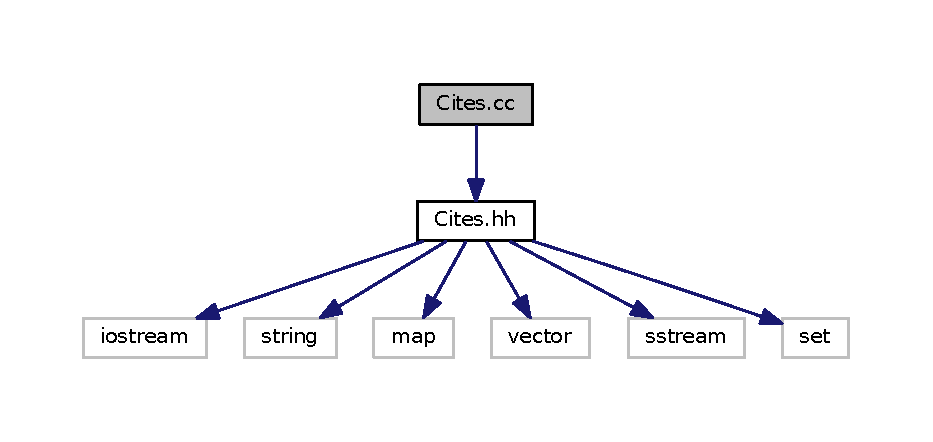
\includegraphics[width=350pt]{_cites_8cc__incl}
\end{center}
\end{figure}

\hypertarget{_cites_8hh}{\section{Referència del Fitxer Cites.\+hh}
\label{_cites_8hh}\index{Cites.\+hh@{Cites.\+hh}}
}


Especificació de la clase \hyperlink{class_cites}{Cites}.  


Inclou el graf de dependències per a Cites.\+hh\+:\nopagebreak
\begin{figure}[H]
\begin{center}
\leavevmode
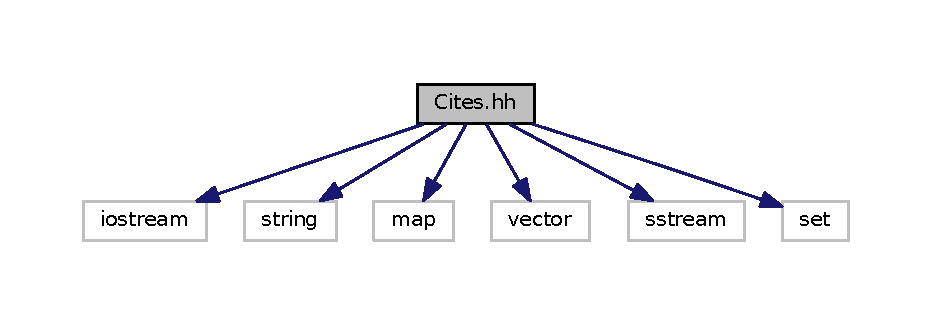
\includegraphics[width=350pt]{_cites_8hh__incl}
\end{center}
\end{figure}
\subsection*{Classes}
\begin{DoxyCompactItemize}
\item 
class \hyperlink{class_cites}{Cites}
\begin{DoxyCompactList}\small\item\em Gestionador de cites. \end{DoxyCompactList}\end{DoxyCompactItemize}


\subsection{Descripció Detallada}
Especificació de la clase \hyperlink{class_cites}{Cites}. 



Definició al fitxer \hyperlink{_cites_8hh_source}{Cites.\+hh}.


\hypertarget{_cjt__autors_8cc}{\section{Referència del Fitxer Cjt\+\_\+autors.\+cc}
\label{_cjt__autors_8cc}\index{Cjt\+\_\+autors.\+cc@{Cjt\+\_\+autors.\+cc}}
}
Inclou el graf de dependències per a Cjt\+\_\+autors.\+cc\+:
\nopagebreak
\begin{figure}[H]
\begin{center}
\leavevmode
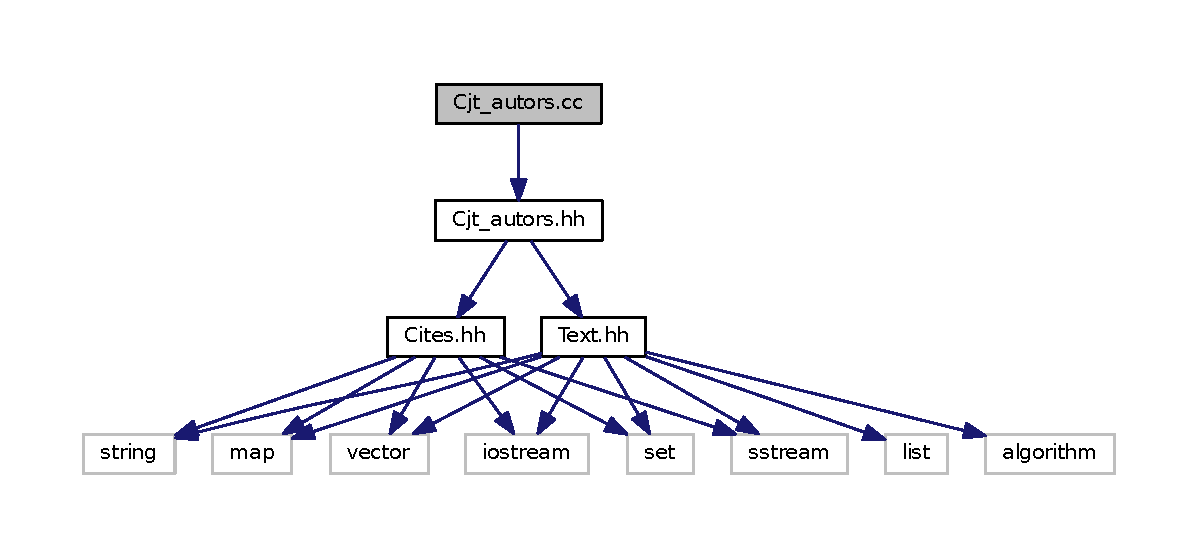
\includegraphics[width=350pt]{_cjt__autors_8cc__incl}
\end{center}
\end{figure}

\hypertarget{_cjt__autors_8hh}{\section{Referència del Fitxer Cjt\+\_\+autors.\+hh}
\label{_cjt__autors_8hh}\index{Cjt\+\_\+autors.\+hh@{Cjt\+\_\+autors.\+hh}}
}


Especificació de la clase \hyperlink{class_cjt__autors}{Cjt\+\_\+autors}.  


Inclou el graf de dependències per a Cjt\+\_\+autors.\+hh\+:
\nopagebreak
\begin{figure}[H]
\begin{center}
\leavevmode
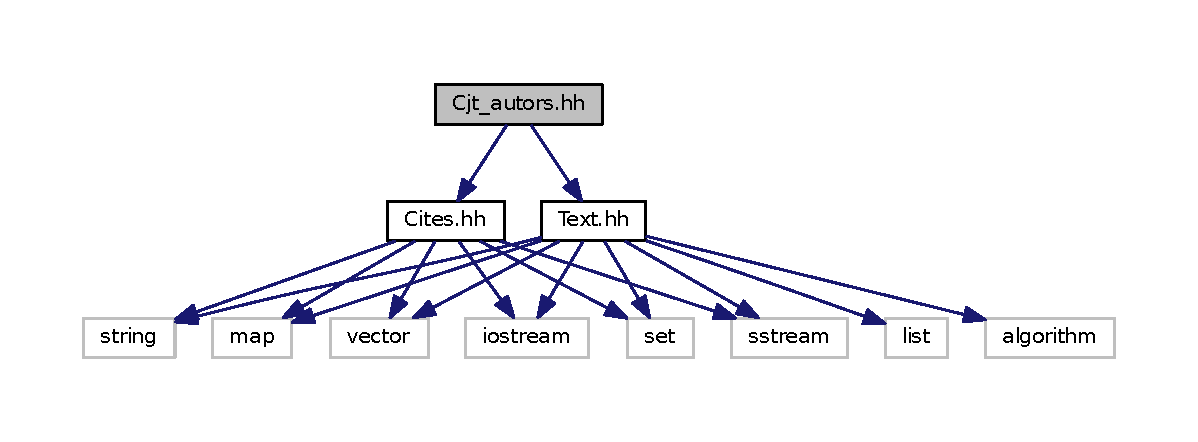
\includegraphics[width=350pt]{_cjt__autors_8hh__incl}
\end{center}
\end{figure}
\subsection*{Classes}
\begin{DoxyCompactItemize}
\item 
class \hyperlink{class_cjt__autors}{Cjt\+\_\+autors}
\begin{DoxyCompactList}\small\item\em Conjunt d'autors amb textos i cites. \end{DoxyCompactList}\end{DoxyCompactItemize}


\subsection{Descripció Detallada}
Especificació de la clase \hyperlink{class_cjt__autors}{Cjt\+\_\+autors}. 



Definició al fitxer \hyperlink{_cjt__autors_8hh_source}{Cjt\+\_\+autors.\+hh}.


\hypertarget{program_8cc}{\section{Referència del Fitxer program.\+cc}
\label{program_8cc}\index{program.\+cc@{program.\+cc}}
}
Inclou el graf de dependències per a program.\+cc\+:
\nopagebreak
\begin{figure}[H]
\begin{center}
\leavevmode
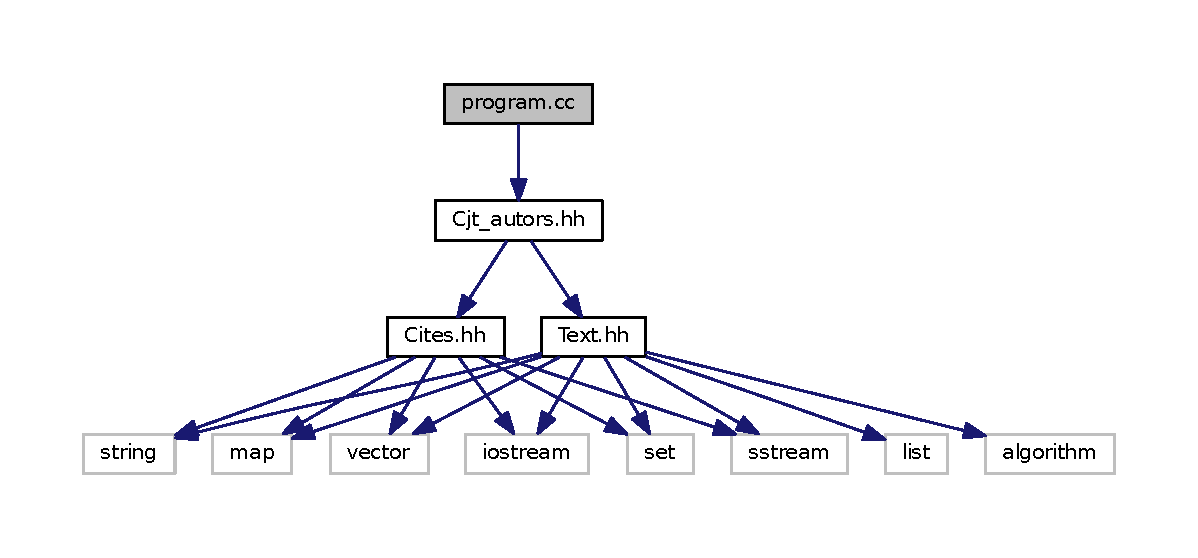
\includegraphics[width=350pt]{program_8cc__incl}
\end{center}
\end{figure}
\subsection*{Funcions}
\begin{DoxyCompactItemize}
\item 
int \hyperlink{program_8cc_ae66f6b31b5ad750f1fe042a706a4e3d4}{main} ()
\end{DoxyCompactItemize}


\subsection{Documentació de les Funcions}
\hypertarget{program_8cc_ae66f6b31b5ad750f1fe042a706a4e3d4}{\index{program.\+cc@{program.\+cc}!main@{main}}
\index{main@{main}!program.\+cc@{program.\+cc}}
\subsubsection[{main}]{\setlength{\rightskip}{0pt plus 5cm}int main (
\begin{DoxyParamCaption}
{}
\end{DoxyParamCaption}
)}}\label{program_8cc_ae66f6b31b5ad750f1fe042a706a4e3d4}


Definició a la línia 5 del fitxer program.\+cc.


\begin{DoxyCode}
5            \{
6     \hyperlink{class_cjt__autors}{Cjt\_autors} cjt\_autors;
7     \textcolor{keywordtype}{string} s;
8     \textcolor{keywordflow}{while} (getline(cin, s) && s != \textcolor{stringliteral}{"sortir"})\{
9         \textcolor{keywordflow}{if}(s[0] != \textcolor{charliteral}{'\(\backslash\)n'} and s[0] != \textcolor{charliteral}{'\(\backslash\)r'} and s.size() != 0)\{
10             cjt\_autors.\hyperlink{class_cjt__autors_a0fb9864fd22881216650552d0697e52d}{comanda}(s);
11             cout << endl;
12         \}
13     \}
14     \textcolor{keywordflow}{return} 0;
15 \}
\end{DoxyCode}

\hypertarget{_text_8cc}{\section{Referència del Fitxer Text.\+cc}
\label{_text_8cc}\index{Text.\+cc@{Text.\+cc}}
}
Inclou el graf de dependències per a Text.\+cc\+:
\nopagebreak
\begin{figure}[H]
\begin{center}
\leavevmode
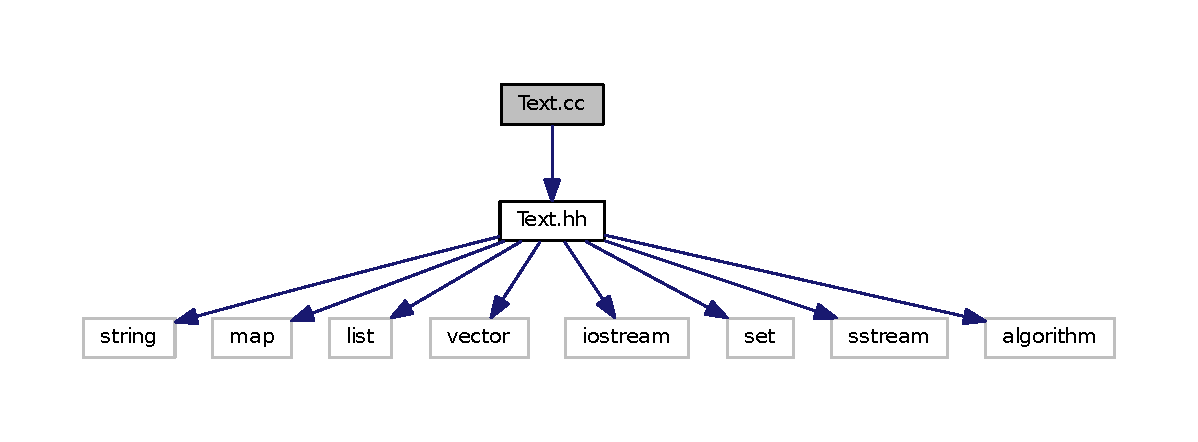
\includegraphics[width=350pt]{_text_8cc__incl}
\end{center}
\end{figure}

\hypertarget{_text_8hh}{\section{Referència del Fitxer Text.\+hh}
\label{_text_8hh}\index{Text.\+hh@{Text.\+hh}}
}


Especificació de la clase \hyperlink{class_text}{Text}.  


Inclou el graf de dependències per a Text.\+hh\+:\nopagebreak
\begin{figure}[H]
\begin{center}
\leavevmode
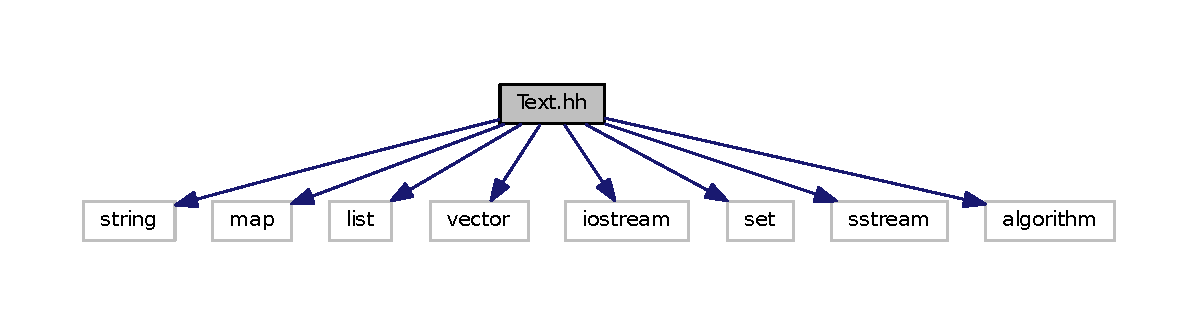
\includegraphics[width=350pt]{_text_8hh__incl}
\end{center}
\end{figure}
\subsection*{Classes}
\begin{DoxyCompactItemize}
\item 
class \hyperlink{class_text}{Text}
\begin{DoxyCompactList}\small\item\em \hyperlink{class_text}{Text}. \end{DoxyCompactList}\end{DoxyCompactItemize}


\subsection{Descripció Detallada}
Especificació de la clase \hyperlink{class_text}{Text}. 



Definició al fitxer \hyperlink{_text_8hh_source}{Text.\+hh}.


%--- End generated contents ---

% Index
\newpage
\phantomsection
\addcontentsline{toc}{chapter}{Índex}
\printindex

\end{document}
